\documentclass[a4paper,14pt]{extarticle} %,twoside

% убрать 6-й вывод

%%%%%%%%%%%%%%%%%%%%%%%%%%%%%%%%%%%%%%%%%%%%%%%%%%%%%%
%%%% Файл упрощённых настроек шаблона диссертации %%%%
%%%%%%%%%%%%%%%%%%%%%%%%%%%%%%%%%%%%%%%%%%%%%%%%%%%%%%

%%%        Подключение пакетов                 %%%
\usepackage{ifthen}                 % добавляет ifthenelse
%%% Инициализирование переменных, не трогать!  %%%
\newcounter{bibliosel}
\newcounter{tabcap}
\newcounter{tablaba}
\newcounter{tabtita}

%%%%%%%%%%%%%%%%%%%%%%%%%%%%%%%%%%%%%%%%%%%%%%%%%%

%%% Область упрощённого управления оформлением %%%

%% Библиография
\setcounter{bibliosel}{0}           % 0 --- встроенная реализация с загрузкой файла через движок bibtex8; 1 --- реализация пакетом biblatex через движок biber

%% Подпись таблиц
\setcounter{tabcap}{0}              % 0 --- по ГОСТ, номер таблицы и название разделены тире, выровнены по левому краю, при необходимости на нескольких строках; 1 --- подпись таблицы не по ГОСТ, на двух и более строках, дальнейшие настройки: 
%Выравнивание первой строки, с подписью и номером
\setcounter{tablaba}{2}             % 0 --- по левому краю; 1 --- по центру; 2 --- по правому краю
%Выравнивание строк с самим названием таблицы
\setcounter{tabtita}{1}             % 0 --- по левому краю; 1 --- по центру; 2 --- по правому краю

               % Упрощённые настройки шаблона 

%%% Проверка используемого TeX-движка %%%
\usepackage{iftex}
\newif\ifxetexorluatex   % определяем новый условный оператор (http://tex.stackexchange.com/a/47579/79756)
\ifXeTeX
    \xetexorluatextrue
\else
    \ifLuaTeX
        \xetexorluatextrue
    \else
        \xetexorluatexfalse
    \fi
\fi

%%% Поля и разметка страницы %%%
\usepackage{pdflscape}                              % Для включения альбомных страниц
\usepackage{geometry}                               % Для последующего задания полей

%%% Математические пакеты %%%
\usepackage{amsthm,amsfonts,amsmath,amssymb,amscd}  % Математические дополнения от AMS
\usepackage{mathtools}                              % Добавляет окружение multlined

%%%% Установки для размера шрифта 14 pt %%%%
%% Формирование переменных и констант для сравнения (один раз для всех подключаемых файлов)%%
%% должно располагаться до вызова пакета fontspec или polyglossia, потому что они сбивают его работу
\newlength{\curtextsize}
\newlength{\bigtextsize}
\setlength{\bigtextsize}{13.9pt}

\makeatletter
%\show\f@size                                       % неплохо для отслеживания, но вызывает стопорение процесса, если документ компилируется без команды  -interaction=nonstopmode 
\setlength{\curtextsize}{\f@size pt}
\makeatother

%%% Кодировки и шрифты %%%
\ifxetexorluatex
    \usepackage{polyglossia}                        % Поддержка многоязычности (fontspec подгружается автоматически)
\else
    \RequirePDFTeX                                  % tests for PDFTEX use and throws an error if a different engine is being used
    \usepackage{cmap}                               % Улучшенный поиск русских слов в полученном pdf-файле
    \usepackage[T2A]{fontenc}                       % Поддержка русских букв
    \usepackage[utf8]{inputenc}                     % Кодировка utf8
    \usepackage[english, russian]{babel}            % Языки: русский, английский
    \IfFileExists{pscyr.sty}{\usepackage{pscyr}}{}  % Красивые русские шрифты
\fi

%%% Оформление абзацев %%%
\usepackage{indentfirst}                            % Красная строка

%%% Цвета %%%
%\usepackage[dvipsnames,usenames]{xcolor}
\usepackage[usenames,dvipsnames]{xcolor}
\usepackage{colortbl}


%%% Таблицы %%%
\usepackage{longtable}                              % Длинные таблицы
\usepackage{multirow,makecell,array}                % Улучшенное форматирование таблиц
\usepackage{booktabs}                               % Возможность оформления таблиц в классическом книжном стиле (при правильном использовании не противоречит ГОСТ)

%%% Общее форматирование
\usepackage{soulutf8}                               % Поддержка переносоустойчивых подчёркиваний и зачёркиваний
\usepackage{icomma}                                 % Запятая в десятичных дробях


%%% Гиперссылки %%%
\usepackage{hyperref}

%%% Изображения %%%
\usepackage{graphicx}                               % Подключаем пакет работы с графикой

%%% Списки %%%
\usepackage{enumitem}

%%% Подписи %%%
\usepackage{caption}                                % Для управления подписями (рисунков и таблиц) % Может управлять номерами рисунков и таблиц с caption %Иногда может управлять заголовками в списках рисунков и таблиц
\usepackage{subcaption}                             % Работа с подрисунками и подобным

%%% Интервалы %%%
\usepackage[onehalfspacing]{setspace}               % Опция запуска пакета правит не только интервалы в обычном тексте, но и формульные

%%% Счётчики %%%
\usepackage[figure,table]{totalcount}               % Счётчик рисунков и таблиц
\usepackage{totcount}                               % Пакет создания счётчиков на основе последнего номера подсчитываемого элемента (может требовать дважды компилировать документ)
\usepackage{totpages}                               % Счётчик страниц, совместимый с hyperref (ссылается на номер последней страницы). Желательно ставить последним пакетом в преамбуле

\usepackage{tabularx}
  % Пакеты общие для диссертации и автореферата
%%% Опционально %%%
% Следующий пакет может быть полезен, если надо ужать текст, чтобы сам текст не править, но чтобы места он занимал поменьше
%\usepackage{savetrees}

% Этот пакет может быть полезен для печати текста брошюрой
%\usepackage[print]{booklet}         % Пакеты для автореферата
\usepackage{tabularx,tabulary}  %таблицы с автоматически подбирающейся шириной столбцов

% Листинги с исходным кодом программ
\usepackage{fancyvrb}
\usepackage{listings}

% Плавающие окружения. во многом лучше пакета float
\usepackage{floatrow}
        % Пакеты для специфических пользовательских задач
%%% Макет страницы %%%
% Выставляем значения полей (ГОСТ 7.0.11-2011, 5.3.7)
\geometry{a4paper,top=2cm,bottom=2cm,left=2.5cm,right=1cm}

%%% Кодировки и шрифты %%%
\ifxetexorluatex
    \setmainlanguage[babelshorthands=true]{russian}  % Язык по-умолчанию русский с поддержкой приятных команд пакета babel
    \setotherlanguage{english}                       % Дополнительный язык = английский (в американской вариации по-умолчанию)
    \ifXeTeX
        \defaultfontfeatures{Ligatures=TeX,Mapping=tex-text}
    \else
        \defaultfontfeatures{Ligatures=TeX}
    \fi
    \setmainfont{Times New Roman}
    \newfontfamily\cyrillicfont{Times New Roman}
    \setsansfont{Arial}
    \newfontfamily\cyrillicfontsf{Arial}
    \setmonofont{Courier New}
    \newfontfamily\cyrillicfonttt{Courier New}
\else
    \IfFileExists{pscyr.sty}{\renewcommand{\rmdefault}{ftm}}{}
\fi

%%% Интервалы %%%
%linespread-реализация ближе к реализации полуторного интервала в ворде.
%setspace реализация заточена под шрифты 10, 11, 12pt, под остальные кегли хуже, но всё же ближе к типографской классике. 
\linespread{1.3}                    % Полуторный интервал (ГОСТ Р 7.0.11-2011, 5.3.6)

%%% Выравнивание и переносы %%%
\sloppy                             % Избавляемся от переполнений
\clubpenalty=10000                  % Запрещаем разрыв страницы после первой строки абзаца
\widowpenalty=10000                 % Запрещаем разрыв страницы после последней строки абзаца

%%% Изображения %%%
\graphicspath{{images/}}            % Пути к изображениям

%%% Подписи %%%
\captionsetup{%
singlelinecheck=off,                % Многострочные подписи, например у таблиц
skip=2pt,                           % Вертикальная отбивка между подписью и содержимым рисунка или таблицы определяется ключом
justification=centering,            % Центрирование подписей, заданных командой \caption
}

%%% Рисунки %%%
\DeclareCaptionLabelSeparator*{emdash}{~--- }             % (ГОСТ 2.105, 4.3.1)
\captionsetup[figure]{labelsep=emdash,font=onehalfspacing,position=bottom}

%%% Таблицы %%%
\ifthenelse{\equal{\thetabcap}{0}}{%
    \newcommand{\tabcapalign}{\raggedright}  % по левому краю страницы или аналога parbox
}

\ifthenelse{\equal{\thetablaba}{0} \AND \equal{\thetabcap}{1}}{%
    \newcommand{\tabcapalign}{\raggedright}  % по левому краю страницы или аналога parbox
}

\ifthenelse{\equal{\thetablaba}{1} \AND \equal{\thetabcap}{1}}{%
    \newcommand{\tabcapalign}{\centering}    % по центру страницы или аналога parbox
}

\ifthenelse{\equal{\thetablaba}{2} \AND \equal{\thetabcap}{1}}{%
    \newcommand{\tabcapalign}{\raggedleft}   % по правому краю страницы или аналога parbox
}

\ifthenelse{\equal{\thetabtita}{0} \AND \equal{\thetabcap}{1}}{%
    \newcommand{\tabtitalign}{\raggedright}  % по левому краю страницы или аналога parbox
}

\ifthenelse{\equal{\thetabtita}{1} \AND \equal{\thetabcap}{1}}{%
    \newcommand{\tabtitalign}{\centering}    % по центру страницы или аналога parbox
}

\ifthenelse{\equal{\thetabtita}{2} \AND \equal{\thetabcap}{1}}{%
    \newcommand{\tabtitalign}{\raggedleft}   % по правому краю страницы или аналога parbox
}

\ifthenelse{\equal{\thetabcap}{0}}{%
    \DeclareCaptionFormat{tablecaption}{\tabcapalign #1#2#3}
    \DeclareCaptionFormat{tablenocaption}{\tabcapalign #1#2}    % Наименование таблицы отсутствует
    \captionsetup[table]{labelsep=emdash}                       % тире как разделитель идентификатора с номером от наименования
}{%
    \DeclareCaptionFormat{tablecaption}{\tabcapalign #1#2\par%  % Идентификатор таблицы на отдельной строке
        \tabtitalign{#3}}                                       % Наименование таблицы строкой ниже
    \DeclareCaptionFormat{tablenocaption}{\tabcapalign #1#2}    % Наименование таблицы отсутствует
    \captionsetup[table]{labelsep=space}                        % пробельный разделитель идентификатора с номером от наименования
}
\captionsetup[table]{format=tablecaption,singlelinecheck=off,font=onehalfspacing,position=top,skip=0pt}  % многострочные наименования и прочее
\DeclareCaptionLabelFormat{continued}{Продолжение таблицы~#2}

%%% Подписи подрисунков %%%
\renewcommand{\thesubfigure}{\asbuk{subfigure}}           % Буквенные номера подрисунков
\captionsetup[subfigure]{font={normalsize},               % Шрифт подписи названий подрисунков (не отличается от основного)
    labelformat=brace,                                    % Формат обозначения подрисунка
    justification=centering,                              % Выключка подписей (форматирование), один из вариантов            
}
%\DeclareCaptionFont{font12pt}{\fontsize{12pt}{13pt}\selectfont} % объявляем шрифт 12pt для использования в подписях, тут же надо интерлиньяж объявлять, если не наследуется
%\captionsetup[subfigure]{font={font12pt}}                 % Шрифт подписи названий подрисунков (всегда 12pt)

%%% Цвета гиперссылок %%%
\definecolor{linkcolor}{rgb}{0.0,0,0.9} % 0.9,0,0
\definecolor{citecolor}{rgb}{0,0.6,0}
\definecolor{urlcolor}{rgb}{0,0,1}

%%% Настройки гиперссылок %%%
\hypersetup{
    linktocpage=true,           % ссылки с номера страницы в оглавлении, списке таблиц и списке рисунков
%    pdfpagelabels=false,        % set PDF page labels (true|false)
    plainpages=false,           % Forces page anchors to be named by the Arabic form  of the page number, rather than the formatted form
    colorlinks,                 % ссылки отображаются раскрашенным текстом, а не раскрашенным прямоугольником, вокруг текста
    linkcolor={linkcolor},      % цвет ссылок типа ref, eqref и подобных
    citecolor={citecolor},      % цвет ссылок-цитат
    urlcolor={urlcolor},        % цвет гиперссылок
}

\ifLuaTeX
    \hypersetup{
        unicode,                % Unicode encoded PDF strings
    }
\fi

%%% Шаблон %%%
\DeclareRobustCommand{\todo}{\textcolor{red}}       % решаем проблему превращения названия цвета в результате \MakeUppercase, http://tex.stackexchange.com/a/187930/79756 , \DeclareRobustCommand protects \todo from expanding inside \MakeUppercase
\setlength{\parindent}{2.5em}                       % Абзацный отступ. Должен быть одинаковым по всему тексту и равен пяти знакам (ГОСТ Р 7.0.11-2011, 5.3.7).

%%% Списки %%%
% Используем дефис для ненумерованных списков (ГОСТ 2.105-95, 4.1.7)
\renewcommand{\labelitemi}{\normalfont\bfseries{--}} 
\setlist{nosep,%                                    % Единый стиль для всех списков (пакет enumitem), без дополнительных интервалов.
    labelindent=\parindent,leftmargin=*%            % Каждый пункт, подпункт и перечисление записывают с абзацного отступа (ГОСТ 2.105-95, 4.1.8)
}
    % Стили общие для диссертации и автореферата
%%% Макет страницы %%%
\oddsidemargin=-13pt
\topmargin=-66pt
\headheight=12pt
\headsep=38pt
\textheight=732pt
\textwidth=484pt
\marginparsep=14pt
\marginparwidth=43pt
\footskip=14pt
\marginparpush=7pt
\hoffset=0pt
\voffset=0pt
%\paperwidth=597pt
%\paperheight=845pt
\parindent=1.5cm                  % Размер табуляции (для красной строки) в начале каждого абзаца
\renewcommand{\baselinestretch}{1.25}

\newcommand{\sfs}{\fontsize{14pt}{15pt}\selectfont}
\sfs % размер шрифта и расстояния между строками

\captionsetup[figure]{name={Рисунок},labelsep=emdash}%period}
           % Стили для автореферата
% \newcounter{pgnum}
% 
% %% Оглавление
% \setcounter{pgnum}{1}               % 0 --- номера страниц никак не обозначены; 1 --- Стр. над номерами страниц (дважды компилировать после изменения)

\usepackage{fancyhdr}
% 
\ifnum\curtextsize>\bigtextsize     % Проверяем условие использования базового шрифта 14 pt
\setlength{\headheight}{17pt}       % Исправляем высоту заголовка
\else
\setlength{\headheight}{15pt}       % Исправляем высоту заголовка
\fi
% 
\headsep=20pt % 38 % 18
% %\footskip=30.0pt % 12 | 17
\topmargin=-53pt % 66 % 51
% 
\makeatletter
\let\ps@plain\ps@fancy              % Подчиняем первые страницы каждой главы общим правилам
\makeatother
\pagestyle{fancy}                   % Меняем стиль оформления страниц
\fancyhf{}                          % Очищаем текущие значения
\fancyhead[C]{\thepage}             % Печатаем номер страницы на середине верхнего поля
\renewcommand{\headrulewidth}{0pt}  % Убираем разделительную линию
% %\makeatother          % Стили для специфических пользовательских задач
%\input{../biblio/bibliopreamble}% Настройки библиографии из внешнего файла (там же выбор: встроенная или на основе biblatex)
%\input{../biblio/biblatex}
%%% Реализация библиографии встроенными средствами посредством движка bibtex8 %%%

%%% Пакеты %%%
\usepackage{cite}                                   % Красивые ссылки на литературу


%%% Стили %%%
%\bibliographystyle{../BibTeX-Styles/utf8gost71u}    % Оформляем библиографию по ГОСТ 7.1 (ГОСТ Р 7.0.11-2011, 5.6.7)
\bibliographystyle{gost705} %705} 

\makeatletter
\renewcommand{\@biblabel}[1]{#1.}   % Заменяем библиографию с квадратных скобок на точку
\makeatother
%% Управление отступами между записями
%% требует etoolbox 
%% http://tex.stackexchange.com/a/105642
%\patchcmd\thebibliography
% {\labelsep}
% {\labelsep\itemsep=5pt\parsep=0pt\relax}
% {}
% {\typeout{Couldn't patch the command}}

%%% Цитирование %%%
\renewcommand\citepunct{;\penalty\citepunctpenalty%
    \hskip.13emplus.1emminus.1em\relax}                % Разделение ; при перечислении ссылок (ГОСТ Р 7.0.5-2008)


%%% Создание команд для вывода списка литературы %%%
\newcommand*{\insertbibliofull}{
\bibliography{../biblio/authorpapers,../biblio/authorconferences,../biblio/literature}         % Подключаем BibTeX-базы % После запятых не должно быть лишних пробелов — он "думает", что это тоже имя пути
}

%\newcommand*{\insertbiblioauthor}{
%\bibliography{../biblio/authorpapersVAK,../biblio/authorpapers,../biblio/authorconferences}         % Подключаем BibTeX-базы % После запятых не должно быть лишних пробелов — он "думает", что это тоже имя пути
%}

%\newcommand*{\insertbiblioother}{
%\bibliography{../biblio/othercites}         % Подключаем BibTeX-базы
%}


%% Счётчик использованных ссылок на литературу, обрабатывающий с учётом неоднократных ссылок
%% Требуется дважды компилировать, поскольку ему нужно считать актуальный внешний файл со списком литературы
\newtotcounter{citenum}
\def\oldcite{}
\let\oldcite=\bibcite
\def\bibcite{\stepcounter{citenum}\oldcite}

%%% Основные сведения %%%
\newcommand{\thesisAuthor}             % Диссертация, ФИО автора
{Петухов Дмитрий Сергеевич}
\newcommand{\thesisUdk}                % Диссертация, УДК
{\todo{621.6-5:[621.65.03:616-78+616.12]}}
\newcommand{\thesisTitle}              % Диссертация, название
{\MakeUppercase{Структурно-параметрическая идентификация имплантируемых роторных насосов крови в аппаратах вспомогательного кровообращения}}%{Разработка и исследование алгоритма идентификации для управления имплантируемым роторным насосом крови в аппаратах вспомогательного кровообращения}}%{Идентификация и управление имплантируемым роторным насосом крови в аппаратах вспомогательного кровообращения}} %Методы и алгоритмы управления работой имплантируемого роторного насоса крови для аппаратов вспомогательного кровообращения}}
%
\newcommand{\thesisSpecialtyNumber}    % Диссертация, специальность, номер
{05.13.01}
\newcommand{\thesisSpecialtyTitle}     % Диссертация, специальность, название
{Системный анализ, управление и обработка информации (технические системы)}
\newcommand{\thesisDegree}             % Диссертация, научная степень
{кандидата технических наук}
\newcommand{\thesisCity}               % Диссертация, город защиты
{Москва}
\newcommand{\thesisYear}               % Диссертация, год защиты
{2018}
\newcommand{\thesisOrganization}       % Диссертация, организация
{в институте биомедицинских систем федерального государственного автономного образовательного учреждения высшего образования <<Национальный исследовательский университет <<Московский институт электронной техники>>}

\newcommand{\supervisorFio}            % Научный руководитель, ФИО
{Селищев Сергей Васильевич,}
\newcommand{\supervisorRegalia}        % Научный руководитель, регалии
{доктор физико-математических наук, профессор}

\newcommand{\opponentOneFio}           % Оппонент 1, ФИО
{Истомина Татьяна Викторовна,}
\newcommand{\opponentOneRegalia}       % Оппонент 1, регалии
{доктор технических наук, профессор,}
\newcommand{\opponentOneJobPlace}      % Оппонент 1, место работы
{ведущий научный сотрудник отдела научных исследований}
\newcommand{\opponentOneJobPost}       % Оппонент 1, должность
{ФГБОУ ВО <<Пензенский государственный технологический университет>>}

\newcommand{\opponentTwoFio}           % Оппонент 2, ФИО
{Беляев Леонид Викторович,}
\newcommand{\opponentTwoRegalia}       % Оппонент 2, регалии
{кандидант технических наук, доцент}
\newcommand{\opponentTwoJobPlace}      % Оппонент 2, место работы
{кафедры <<Технология машиностроения>>}
\newcommand{\opponentTwoJobPost}       % Оппонент 2, должность
{ФГБОУ ВО <<Владимирский государственный университет им. А. Г. и Н. Г. Столетовых>>}

\newcommand{\leadingOrganizationTitle} % Ведущая организация, дополнительные строки
{Федеральное государственное бюджетное образовательное учреждение высшего образования <<Юго-Западный Государственный Университет>>}

\newcommand{\defenseDate}              % Защита, дата
{\todo{DD mmmm 2018~г.~в~XX часов}}
\newcommand{\defenseCouncilNumber}     % Защита, номер диссертационного совета
{Д 212.134.06}
\newcommand{\defenseCouncilTitle}      % Защита, учреждение диссертационного совета
{Национальном исследовательском университете <<МИЭТ>>}
\newcommand{\defenseCouncilAddress}    % Защита, адрес учреждение диссертационного совета
{124498, г. Москва, г. Зеленоград, площадь Шокина, д. 1}

\newcommand{\defenseSecretaryFio}      % Секретарь диссертационного совета, ФИО
{Гуреев Александр Васильевич}
\newcommand{\defenseSecretaryRegalia}  % Секретарь диссертационного совета, регалии
{доктор технических наук, доцент}            % Для сокращений есть ГОСТы, например: ГОСТ Р 7.0.12-2011 + http://base.garant.ru/179724/#block_30000

\newcommand{\synopsisLibrary}          % Автореферат, название библиотеки
{[URL: https://www.miet.ru/dis/]}
\newcommand{\synopsisDate}             % Автореферат, дата рассылки
{\todo{DD mmmmmmmm 2018 г}}      % Основные сведения

\usepackage{tikz}
\usetikzlibrary{arrows,positioning}
\usetikzlibrary{shapes.geometric,calc,chains}
\usetikzlibrary{arrows.meta}

% -------------------------------- Bibliography 
%\NewBibliographyString{langjapanese}
%\NewBibliographyString{fromjapanese}

%\usepackage{layout}
%\usepackage{showframe}

\begin{document}

%\layout{}

% Титульный лист (ГОСТ Р 7.0.11-2001, 5.1)
\thispagestyle{empty}%
\begin{center}%
\MakeUppercase{Федеральное государственное автономное образовательное учреждение высшего образования <<Национальный исследовательский университет <<Московский институт электронной техники>>}
\end{center}%
%
\vspace{0pt plus4fill} %число перед fill = кратность относительно некоторого расстояния fill, кусками которого заполнены пустые места
\begin{flushright}%
  {На правах рукописи}\\\vskip5pt
  
\includegraphics[height=2.6cm]{../images/my_signature} 
\end{flushright}%
\vspace{-\baselineskip}
\vspace{-\baselineskip}

\vspace{0pt plus6fill} %число перед fill = кратность относительно некоторого расстояния fill, кусками которого заполнены пустые места
\begin{center}%
{\thesisAuthor}
\end{center}%
%
\vspace{0pt plus1fill} %число перед fill = кратность относительно некоторого расстояния fill, кусками которого заполнены пустые места
\begin{center}%
\textbf{СТРУКТУРНО-ПАРАМЕТРИЧЕСКАЯ ИДЕНТИФИКАЦИЯ ИМПЛАНТИРУЕМЫХ РОТОРНЫХ НАСОСОВ КРОВИ В \\ АППАРАТАХ ВСПОМОГАТЕЛЬНОГО КРОВООБРАЩЕНИЯ}

\vspace{0pt plus2fill} %число перед fill = кратность относительно некоторого расстояния fill, кусками которого заполнены пустые места
\vspace{\baselineskip}
{%\small
\thesisSpecialtyNumber~---~Системный анализ, управление и обработка информации \\(технические системы) %\thesisSpecialtyTitle
}

\vspace{0pt plus2fill} %число перед fill = кратность относительно некоторого расстояния fill, кусками которого заполнены пустые места
Диссертация на соискание ученой степени

\thesisDegree
\end{center}%
%
\vspace{0pt plus4fill} %число перед fill = кратность относительно некоторого расстояния fill, кусками которого заполнены пустые места
\begin{flushright}%
Научный руководитель:

д.ф.-м.н., профессор С. В. Селищев %\supervisorRegalia

%\supervisorFio
\end{flushright}%
%
\vspace{0pt plus4fill} %число перед fill = кратность относительно некоторого расстояния fill, кусками которого заполнены пустые места
\begin{center}%
{\thesisCity~--- \thesisYear}
\end{center}%
\newpage
           % Титульный лист
\subsection*{Общая характеристика работы}

\newcommand{\actuality}{\underline{\textbf{Актуальность темы исследования.}}}
\newcommand{\aim}{\underline{\textbf{Целью}}}
\newcommand{\tasks}{\underline{\textbf{задачи}}}
\newcommand{\defpositions}{\underline{\textbf{Положения, выносимые на~защиту:}}}
\newcommand{\novelty}{\underline{\textbf{Научная новизна:}}}
\newcommand{\influence}{\underline{\textbf{Практическая значимость:}}}
\newcommand{\methodology}{\underline{\textbf{Методы исследования.}}}
\newcommand{\reliability}{\underline{\textbf{Достоверность}}}
\newcommand{\probation}{\underline{\textbf{Апробация результатов.}}}
\newcommand{\contribution}{\underline{\textbf{Личный вклад.}}}
\newcommand{\implement}{\underline{\textbf{Внедрение результатов.}}}
\newcommand{\publications}{\underline{\textbf{Публикации.}}}
\newcommand{\structure}{\underline{\textbf{Структура и объем работы.}}}

{\actuality}

%%%
% Роторные насосы являются сложной системой и находят применение в различных областях (еще сложнее когда качают кровь)
% Необходима идентификация для определения параметров насоса
%%%

В настоящее время аппараты вспомогательного кровообращения (АВК) успешно применяются при лечении различных форм сердечной недостаточности. Основным элементом АВК является имплантируемый роторный насос крови (РНК), который является сложной технической системой, помогающей поддерживать кровообращение в сердечно-сосудистой системе. Основным параметром РНК является скорость вращения ротора, от которой зависит степень поддержки кровообращения.

% Сердечная недостаточность (СН) является тяжелым, прогрессирующим заболеванием, которое характеризуется неспособностью сердца перекачивать кровь в объеме, достаточном для обеспечения метаболических потребностей организма. На данный момент наиболее эффективным способом лечения тяжелых форм сердечной недостаточности является трансплантация сердца. 
% 
% Вследствие дефицита донорских сердец для трансплантации в последние десять лет активное развитие получили аппараты вспомогательного кровообращения (АВК), используемые для лечения пациентов с различными формами СН. Основным компонентом данных аппаратов является имплантируемый роторный насос крови (РНК), который благодаря непрерывному вращению ротора помогает поддерживать необходимый уровень кровообращения. 

Одним из ключевых направлений развития технологии вспомогательного кровообращения, позволяющим повысить эффективность лечения сердечной недостаточности, является управление имплантируемым РНК. В литературе предложено множество способов управления РНК с использованием скорости вращения ротора в качестве управляемой переменной. Для управления имплантируемыми роторными насосами крови необходима их идентификация, то есть построение математической модели по результатам экспериментальных исследований. Изучению проблемы идентификации сложных технических систем посвящен целый ряд фундаментальных исследований российских и зарубежных авторов: Д. Гроппа, Л. Льюнга, С. А. Акулова и А. А. Федотова, В. М. Трояновского и др. [1--4]. %результатам экспериментального исследования. 

В настоящее время решением проблемы идентификации насосов, в том числе имплантируемых роторных насосов крови, занимается большое количество исследователей. Значительный вклад в исследования и практическое применение полученных результатов был внесен такими учеными, как Г. П. Иткин, К. Н. Дозоров, Ю. В. Солодянников, А. Б. Тмур, F. Moscato, T. Pirbodaghi и др. [5--10].% Работы данных исследователей в большинстве случаев направлены на построение математических моделей точно аппроксимирующих экспериментальные данные и не анализируют эффективность управления имплантируемыми роторными насосами крови. 

% В то же время не существует универсального способа идентификации имплантируемых РНК, что обусловлено их многообразием, сложным устройством, зависимостью производительности насосов от состояния сердечно-сосудистой системы и, как следствие, строгим требованием учитывать взаимодействие насосов с сердечно-сосудистой системой. %Вместе с этим, работы по идентификации имплантируемых РНК, как правило, направлены на повышение точности аппроксимации исходных экспериментальных данных математической моделью, и не проводят исследования эффективности управления имплантируемыми роторными насосами крови. % рассматривают эффективность управления имплантируемыми роторными насосами крови.

Идентификация имплантируемых роторных насосов крови остается сложной задачей и в настоящее время не существует универсального и общепринятого способа идентификации. Это обусловлено многообразием и сложным устройством роторных насосов крови, зависимостью производительности насосов от состояния сердечно-сосудистой системы и, как следствие, строгим требованием учитывать взаимодействие насосов с сердечно-сосудистой системой. Исследования по идентификации роторных насосов крови направлены на построение математических моделей точно аппроксимирующих экспериментальные данные, при этом необходимым является исследование эффективности идентификации для управления роторными насосами крови с использованием построенных математических моделей.

%В то же время не существует общепринятого и универсального алгоритма идентификации, что обусловлено сложностью описания работы имплантируемого роторного насоса и непрерывным взаимодействием сердечно-сосудистой системы и насоса, которые образуют сложную систему. 

Таким образом, актуальной является задача идентификации имплантируемых роторных насосов крови с использованием универсального алгоритма, что требует структурной идентификации, которая заключается в представлении объекта управления в виде математической модели с определением ее структуры, и параметрической идентификации, которая заключается в определении числовых значений коэффициентов математической модели согласно экспериментальным данным, с последующим исследованием и оценкой эффективности идентификации для управления имплантируемыми роторными насосами крови в аппаратах вспомогательного кровообращения.

% Таким образом, для повышения эффективности лечения пациентов с сердечной недостаточностью посредством аппаратов вспомогательного кровообращения еобходима разработка подходов к регулированию работы РНК, обеспечивающих возможность диагностики состояния сердечно-сосудистой системы и автоматизированное регулирование параметров АВК с целью поддержания определенных уровней производительности РНК или состояний в сердечно-сосудистой системе.
% 
%  Настоящая работа посвящена разработке методов и алгоритмов управления работой имплантируемого роторного насоса крови для аппаратов вспомогательного кровообращения. Предполагается, что они позволят разрешить указанные проблемы и предотвратить физиологические нарушения при экплуатации АВК, что в долгосрочной перспективе должно привести к улучшению результатов лечения. 
% 
% -----------------------------------------------------------------------------------------------------------------------------------
% -----------------------------------------------------------------------------------------------------------------------------------

\textbf{Объектом исследования} являются имплантируемые роторные насосы крови в аппаратах вспомогательного кровообращения.

\textbf{Предметом исследования} являются методы и алгоритмы структурно-параметрической идентификации имплантируемых роторных насосов крови в аппаратах вспомогательного кровообращения.

\textbf{Проблемная ситуация, сложившаяся в области объекта исследований}, определяется тем, что идентификация имплантируемых роторных насосов крови в аппаратах вспомогательного кровообращения является сложной и актуальной научно-технической задачей, которая требует разработки методов и алгоритмов структурной и параметрической идентификации, обеспечивающих высокую эффективность управления имплантируемыми роторными насосами крови в аппаратах вспомогательного кровообращения. 

Обобщенная схема поддержки кровообращения с помощью АВК приведена на рисунке \ref{img:system_links}. Взаимодействие АВК с телом пациента представлено взаимодействием РНК, крови, сосудов и сердца; основными параметрами данной системы являются расход насоса $Q(t)$ и перепад давления в насосе $H(t)$, которые зависят от скорости вращения ротора насоса $\omega(t)$. % отражает состояние сердечно-сосудистой системы и взаимосвязан с $Q(t)$ и $\omega(t)$. 

\begin{figure}[ht]
  \begin{minipage}[ht]{0.43\linewidth}
    \center{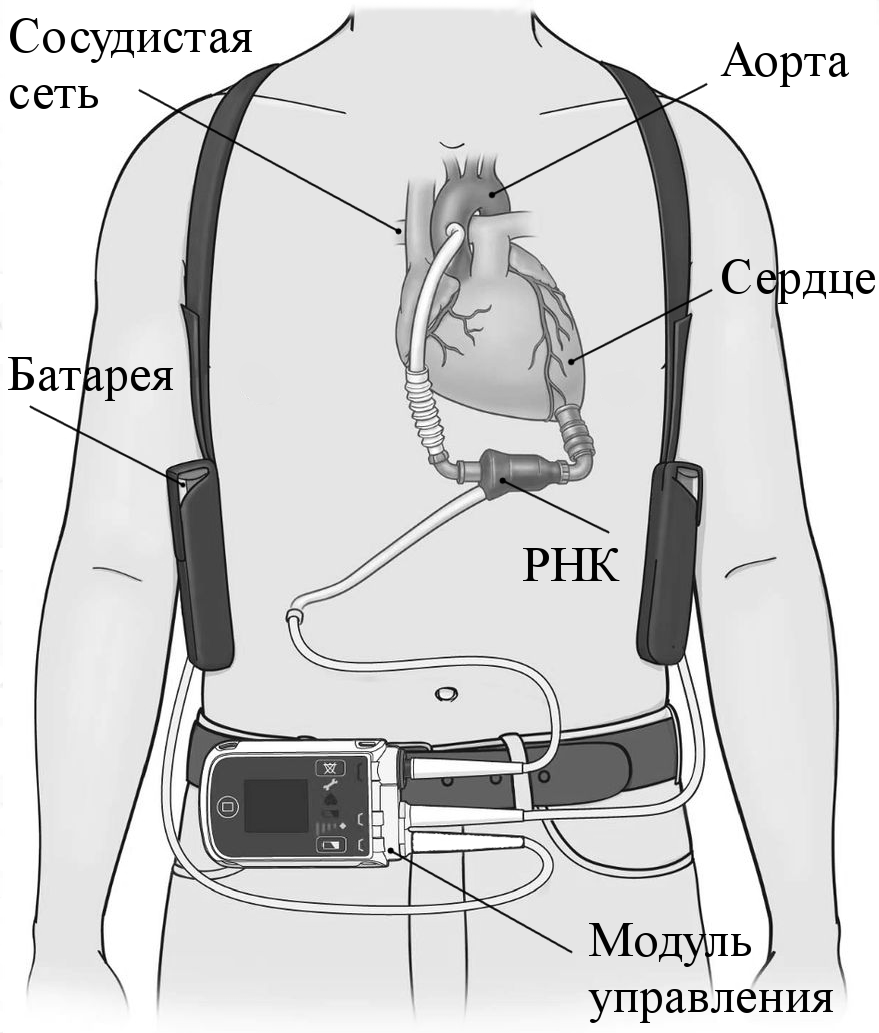
\includegraphics [scale=0.9] {../images/vad_system_abs}}
  \end{minipage}
  \hfill
  \begin{minipage}[ht]{0.55\linewidth}
    \center{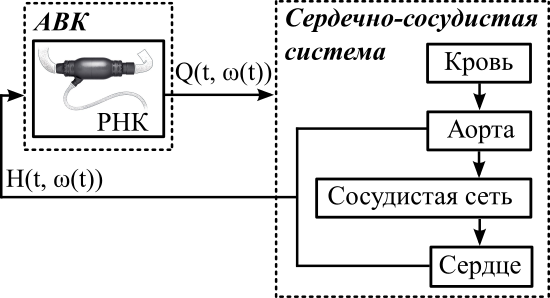
\includegraphics [scale=1.85] {../images/system_links}}
  \end{minipage}
  \caption{Представление аппарата вспомогательного кровообращения (АВК) в виде системы, образованной роторным насосом крови (РНК) и сердечно-сосудистой системой; $Q(t)$ -- расход насоса, $\omega(t)$ -- скорость вращения ротора насоса, $H(t)$ -- перепад давления в насосе, $t$ -- время}
  \label{img:system_links}  

\begin{tikzpicture}[node distance=1cm, overlay]  
\tikzstyle{arrow} = [thick,->,>=stealth]
\draw [arrow] (6.4, 6.3) |- (7.6, 6.3);
\draw [arrow] (7.4, 5.6) |- (6.2, 5.6);
\end{tikzpicture} 

\end{figure}

% В левой части рисунка \ref{img:system_links} представлена схема взаимодействия АВК и тела пациента; в правой части -- процесс взаимодействия АВК и сердечно-сосудистой системы при помощи РНК. При этом расход насоса $Q(t)$ определяется скоростью вращения ротора $\omega(t)$ и взаимосвязан с параметрами сердечно-сосудистой системы.

% При этом также возникает необходимость разработки методов и алгоритмов идентификации таких систем.

 \aim\ диссертационной работы является разработка и исследование способов структурно-параметрической идентификации имплантируемых роторных насосов крови для повышения эффективности идентификации и управления имплантируемыми роторными насосами крови в аппаратах вспомогательного кровообращения.

%разработка и исследование алгоритма идентификации для управления имплантируемым роторным насосом крови в аппаратах вспомогательного кровообращения.

% идентификация и управление имплантируемым роторным насосом крови в аппаратах вспомогательного кровообращения.
% \newpage
В~соответствии с целью диссертационной работы поставлены следующие {\tasks}:
\begin{enumerate}
  \item Разработка математической модели идентификации имплантируемого роторного насоса крови на основе расходно-напорных характеристик.
  \item Разработка математической модели сердечно-сосудистой системы с учетом имплантации роторного насоса крови.
  \item Исследование взаимодействия имплантируемого роторного насоса крови и сердечно-сосудистой системы методами математического моделирования и анализ результатов исследования с целью повышения эффективности идентификации и управления имплантируемым роторным насосом крови.
  \item Исследование взаимодействия имплантируемого роторного насоса крови и сердечно-сосудистой системы с использованием экспериментальных данных для роторных насосов крови Спутник с целью верификации результатов математического моделирования.
%   \item Разработать алгоритм идентификации имплантируемого роторного насоса крови на основе расходно-напорных характеристик, полученных в результате экспериментального исследования имплантируемых роторных насосов крови и опубликованных в литературе.
%   \item Исследовать разработанный алгоритм идентификации имплантируемого роторного насоса крови с использованием математической модели сердечно-сосудистой системы. % возможности алгоритма для управления имплантируемым роторным насосом крови с помощью моделирования взаимодействия  роторного насоса и сердечно-сосудистой системы в условиях сердечной недостаточности. % можно описать раздельно или переформулировать
%   \item Исследовать разработанный алгоритм идентификации с использованием результатов экспериментального исследования имплантируемых роторных насосов крови <<Спутник>> в испытательном гидродинамическом стенде.
%   \item Разработать способ управления имплантируемым роторным насосом крови на основе результатов исследования алгоритма идентификации. 
\end{enumerate}

% -----------------------------------------------------------------------------------------------------------------------------------
% -----------------------------------------------------------------------------------------------------------------------------------
\newpage
\novelty
\begin{enumerate}
  % что нового в разработке, исследовании и управлении?
  \item Разработан алгоритм структурно-параметрической идентификации, который позволяет построить математическую модель в соответствии с критериями оценки эффективности идентификации для управления имплантируемыми роторными насосами крови. \\На основе построенной математической модели разработан способ управления имплантируемым роторным насосом крови, направленный на поддержание заданного уровня расхода насоса и предотвращение следующих нежелательных режимов работы насоса: обратное течение через насос, полная разгрузка желудочка сердца и коллапс желудочка сердца.
  \item Предложены следующие критерии, которые позволяют оценить эффективность идентификации для управления имплантируемыми роторными насосами крови: точность оценки расхода насоса и точность определения перехода между режимами работы насоса. \\С использованием алгоритма структурно-параметрической идентификации и в соответствии с предложенными критериями оценки эффективности идентификации построены математические модели имплантируемых роторных насосов крови Спутник.
  \item В результате комплексного исследования взаимодействия имплантируемого роторного насоса крови и сердечно-сосудистой системы на основе математической модели идентификации разработан метод определения следующих режимов работы имплантируемого роторного насоса крови: обратное течение через насос, частичная и полная разгрузка желудочка сердца, и коллапс желудочка сердца.
\end{enumerate}

% -----------------------------------------------------------------------------------------------------------------------------------
% -----------------------------------------------------------------------------------------------------------------------------------

\influence\ 
\begin{enumerate}
 \item Разработанные программные средства использованы при моделировании взаимодействия имплантируемого роторного насоса крови и сердечно-сосудистой системы и теоретическом исследовании имплантируемых роторных насосов крови Спутник. 
 \item Разработанный алгоритм структурно-параметрической идентификации может быть использован для управления имплантируемыми роторными насосами крови при проведении экспериментальных исследований в испытательных гидродинамических стендах. % напиши конкретно на ком и на чем
\end{enumerate}

% -----------------------------------------------------------------------------------------------------------------------------------
% -----------------------------------------------------------------------------------------------------------------------------------

\underline{\textbf{Личный вклад автора.}}

Автор принимал активное и непосредственное участие в выполнении всех работ, которые легли в основу диссертации.

\defpositions

\begin{enumerate}
  % с требуемой точностью % обеспечивает следующие возможности для управления: оценка расхода насоса и определение режимов работы насоса. %\vskip5pt
  %\item Разработан алгоритм идентификации, который позволяет повысить эффективность управления имплантируемым роторным насосом крови в аппаратах вспомогательного кровообращения.
 % \item Разработанный метод определения режимов работы имплантируемого роторного насоса крови позволяет определять следующие переходы между режимами работы насоса, что подтверждается результатами моделирования и исследования с использованием экспериментальных данных для роторных насосов крови Спутник: обратное течение через насос, частичная и полная разгрузка желудочка сердца, и коллапс желудочка сердца. %, что подтверждается результатами моделирования и исследования с использованием экспериментальных данных.
 \item Предложены критерии, которые позволяют оценить эффективность идентификации для управления имплантируемыми роторными насосами крови в аппаратах вспомогательного кровообращения.
  \item Разработанный алгоритм структурно-параметрической идентификации позволяет построить математические модели имплантируемых роторных насосов крови в соответствии с критериями оценки эффективности идентификации.
  \item Построенные математические модели имплантируемых роторных насосов крови позволяют определить переходы между следующими режимами работы насоса: обратное течение через насос, частичная и полная разгрузка желудочка сердца, и коллапс желудочка сердца.
  \item Разработанный способ управления имплантируемым роторным насосом крови позволяет поддерживать заданный уровень расхода насоса и предотвращать следующие нежелательные режимы работы насоса: обратное течение через насос, полная разгрузка желудочка сердца и коллапс желудочка сердца. 
 %, что позволяет повысить эффективность управления насосом в аппаратах вспомогательного кровообращения.
  %\item Разработанная модель идентификации имплантируемого роторного насоса крови позволяет описать расходно-напорные характеристики с требуемым уровнем точности. 
\end{enumerate}

% \begin{enumerate}
%   \item Разработанная математическая модель имплантируемого роторного насоса крови позволяет учесть влияние вязкости и инерции жидкости на расходно-напорные характеристики роторного насоса крови.
%   \item Разработанный метод определения режимов работы насоса позволяет с высокой точностью определить режимы работы насоса посредством анализа динамики течения жидкости через насос с помощью математической модели роторного насоса крови. %исследования на математической модели сердечно-сосудистой системы и результатами верификации с использованием данных экспериментального исследования. 
%   \item Разработанный алгоритм управления работой имплантируемого роторного насоса крови обеспечивает соответствие основным требованиям к управлению работой имплантируемого роторного насоса крови для аппаратов вспомогательного кровообращения.
%   \item Предложенный алгоритм разработки математической модели имплантируемого роторного насоса крови на основе результатов экспериментального исследования роторного насоса крови позволяет обеспечить высокую точность оценки расхода насоса и определения режимов работы насоса.
% \end{enumerate}


% -----------------------------------------------------------------------------------------------------------------------------------
% -----------------------------------------------------------------------------------------------------------------------------------

\methodology\ % Основными методами исследования в диссертационной работе являются методы математического моделирования и оптимизации. %Экспериментальное исследование выполнено \textit{in vitro} в испытательном гидродинамическом стенде. % программных библиотек
%Обоснованность результатов моделирования подтверждена данными экспериментальных исследований на гидродинамическом стенде.

% пиши конкретно: экспериментальное исследование чего? методы исследования можно отразить в задачах работы

Методами исследования диссертационной работы являются методы системного анализа и математического моделирования. 

%Обработка и анализ данных выполнены с использованием языка программирования Python.
%Идентификация имплантируемых роторных насосов крови проведена с использованием алгоритмов оптимизации Левенберга-Марквардта и дифференциальной эволюции. 

% -----------------------------------------------------------------------------------------------------------------------------------
% -----------------------------------------------------------------------------------------------------------------------------------

\reliability\ полученных результатов обусловлена корректностью поставленных задач, комплексным характером проведенных исследований и согласием полученных результатов с литературными данными. %литературными данными и результатами экспериментального исследования. 

%использованием апробированных методов моделирования
%использованием проверенных подходов к моделированию динамики кровообращения

% -----------------------------------------------------------------------------------------------------------------------------------
% -----------------------------------------------------------------------------------------------------------------------------------

\probation\
Основные результаты диссертационной работы были представлены на следующих конференциях: % докладывались

\begin{itemize}
 \item 44th Annual ESAO and 7th IFAO Congress (г. Вена, Австрия, 2017),
 \item 2nd International Symposium <<Physics, Engineering and Technologies for Biomedicine>> (г. Москва, 2017),
 \item 20-23-я всероссийская конференция <<Микроэлектроника и информатика>> (г. Москва, 2013 -- 2016),
 \item 61-62nd ASAIO Annual Conference (г. Чикаго, США, 2015; г. Сан-Франциско, США, 2016),
 \item 24th Congress of the International Society for Rotary Blood Pumps (г. Мито, Япония, 2016),
 \item X-XI German-Russian Conference on Biomedical Engineering (г. Санкт-Петербург, 2014; г. Ахен, Германия, 2015),
 \item 42th Annual ESAO Congress (г. Лёвен, Бельгия, 2015),
 \item 37th Annual International Conference of the IEEE Engineering in Medicine and Biology Society (г. Милан, Италия, 2015),
 \item 16-я научно-техническая конференция <<МедТех>> (о. Кефалония, Греция, 2014),
 \item 11-я международная конференция <<Физика и радиоэлектроника в медицине и экологии>> (г. Суздаль, 2014),
 \item 6-я Троицкая конференция <<Медицинская физика и инновации в медицине>> (г. Троицк, 2014).
\end{itemize}

\implement\
Результаты диссертационной работы получены в рамках следующих проектов и исследований:

\begin{itemize}
 \item проект Российского научного фонда № 14-39-00044 <<Разработка адаптивной системы вспомогательного кровообращения с целью персонализации лечения острой формы сердечной недостаточности>> (2014 -- 2016 гг.) по приоритетному направлению <<Проведение фундаментальных научных исследований и поисковых научных исследований вновь создаваемыми научной организацией и вузом совместными научными лабораториями>>,
 \item прикладные научные исследования в рамках ФЦП <<Исследования и разработки по приоритетным направлениям развития научно-технологического комплекса России на 2014 – 2020 годы>> по теме <<Разработка аппарата длительного механического замещения функции сердца>> (RFMEFI57814X0057) (2014 -- 2016 гг.),
 \item прикладные научные исследования и экспериментальные разработки в рамках ФЦП <<Исследования и разработки по приоритетным направлениям развития научно-технологического комплекса России на 2014 – 2020 годы>> по теме <<Миниатюризация имплантируемых насосов крови для их применения в педиатрической кардиохирургии>> (RFMEFI58115X0014) (2015 -- 2017 гг.).
\end{itemize}

Результаты работы внедрены в учебный процесс института биомедицинских систем Национального исследовательского университета <<МИЭТ>> в рамках дисциплины <<Биомедицинская инженерия искусственных органов>> для магистров, обучающихся по направлению 12.04.04 <<Биотехнические системы и технологии>>.

%Российского научного фонда и Министерства образования и науки РФ в рамках ФЦП <<Исследования и разработки по приоритетным направлениям развития научно-технологического комплекса России на 2014 – 2020 годы>>.

%Результаты диссертационной работы использованы при реализации следующих проектов кафедры биомедицинских систем Национального исследовательского университета «МИЭТ»: 

%Исследования поддержаны Министерством образования и науки РФ в рамках ФЦП <<Исследования и разработки по приоритетным направлениям развития научно-технологического комплекса России на 2014 – 2020 годы>> по теме <<Разработка аппарата длительного механического замещения функции сердца>> (RFMEFI57814X0057) на 2014 -- 2016 г. и теме <<Миниатюризация имплантируемых насосов крови для их применения в педиатрической кардиохирургии>> (RFMEFI58115X0014) на 2015 -- 2017 г., и Российским научным фондом по теме <<Разработка адаптивной системы вспомогательного кровообращения с целью персонализации лечения острой формы сердечной недостаточности>> (проект № 14-39-00044) на 2014 -- 2016 г.

%\contribution\ Автор принимал активное участие \ldots № 14.578.21.0057 (RFMEFI57814X0057)  № 14.581.21.0014 (RFMEFI58115X0014) 

% -----------------------------------------------------------------------------------------------------------------------------------
% -----------------------------------------------------------------------------------------------------------------------------------

\publications\ Результаты по теме диссертации изложены в 29 научных работах, из них 11 опубликованы в рецензируемых научных изданиях, входящих в перечень Высшей аттестационной комиссии при Министерстве образования и науки Российской Федерации и в международную реферативную базу данных Scopus, 18 -- в тезисах докладов всероссийских и международных конференций. % По теме диссертации опубликована 21 научная работа, из них 8 изданы в журналах, 
 % Характеристика работы по структуре во введении и в автореферате не отличается (ГОСТ Р 7.0.11, пункты 5.3.1 и 9.2.1), потому её загружаем из одного и того же внешнего файла, предварительно задав форму выделения некоторым параметрам

%\underline{\textbf{Объем и структура работы.}} Диссертация состоит из~введения, четырех глав, заключения и~приложения. Полный объем диссертации \textbf{ХХХ}~страниц текста с~\textbf{ХХ}~рисунками и~5~таблицами. Список литературы содержит \textbf{ХХX}~наименование.

\structure\ Диссертационная работа состоит из введения, четырех глав, заключения, списка литературы и трех приложений. Полный объем работы составляет 132 страницы текста с 44 рисунками и 11 таблицами. Список литературы содержит 150 наименований. 

%\newpage
\subsection*{Содержание работы}

\underline{\textbf{Во введении}} обоснована актуальность темы исследования, сформулированы цель работы, научная новизна и практическая значимость полученных результатов, представлены положения, выносимые на защиту.

% -----------------------------------------------------------------------------------------------------------------------------------------------------------------------------------------
% -----------------------------------------------------------------------------------------------------------------------------------------------------------------------------------------

\underline{\textbf{В первой главе}} рассмотрена история развития имплантируемых роторных насосов крови (РНК) в аппаратах вспомогательного кровообращения (АВК), продемонстрировано многообразие имплантируемых роторных насосов крови, применяемых в современной клинической практике.

Представлен аналитический обзор литературных источников, посвященных проблеме идентификации имплантируемых роторных насосов крови. Актуальной данную проблему делает многообразие роторных насосов крови, их сложное взаимодействие с сердечно-сосудистой системой.

Рассмотрены различные структуры математических моделей, полученные в результате идентификации, описано применение математических моделей для управления имплантируемыми РНК в аппаратах вспомогательного кровообращения.

% Выделены следующие типы управления: управление, направленное на поддержание заданного уровня расхода, и управление, направленное на предотвращение нежелательных состояний в сердечно-сосудистой системе, таких как коллапс желудочка сердца. Наиболее распространенным является первый тип управления.

Выявлено, что не существует универсального и общепринятого алгоритма идентификации, таким образом задача идентификации решается индивидуально для каждого насоса. Отмечено, что идентификация в общем случае направлена на повышение точности аппроксимации исходных экспериментальных данных математической моделью; построенные в результате идентификации математические модели, как правило, применяются для управления расходом имплантируемого роторного насоса крови.

Известная работа по идентификации имплантируемого РНК [9] заключается в параметрической идентификации и не исследует влияние изменений в структуре математической модели на точность аппроксимации экспериментальных данных или эффективность управления. Таким образом, недостаточное внимание уделяется исследованию структуры математической модели, а также применению идентифицированной математической модели к управлению имплантируемыми роторными насосами крови в аппаратах вспомогательного кровообращения.

Отмечено, что для корректной идентификации необходимо учесть взаимодействие насосов с сердечно-сосудистой системой, что требует проведения комплексного исследования, которое должно привести к повышению эффективности идентификации и управления имплантируемыми РНК.

% Помимо этого рассмотрена проблема идентификации имплантируемых РНК, т.\:е. построения математических моделей по экспериментальным данным; проведен сравнительный анализ способов идентификации РНК. Указано, что для корректной идентификации требуется учесть взаимодействие насосов с сердечно-сосудистой системой. 


% насосов крови необходимо учитывать взаимодействие насоса и сердечно-сосудистой системы, которые образуют сложную систему. 

%При этом проведен анализ подходов к идентификации РНК, а также рассмотрены  возможности для управления РНК, которые обеспечивают построенные в результате идентификации математические модели.  

% Рассматриваются различные подходы к идентификации, описанные в работах.  Указывается, что все подходы различны и нет единого или универсального способа идентификации, что обусловлено тем-то (сложность идентификации - насосы разные).

% -----------------------------------------------------------------------------------------------------------------------------------------------------------------------------------------
% -----------------------------------------------------------------------------------------------------------------------------------------------------------------------------------------

\underline{\textbf{Во второй главе}} описывается разработка математической модели идентификации имплантируемого роторного насоса крови и математической модели сердечно-сосудистой системы с учетом имплантации РНК.

Первоначально решалась задача идентификации на основе расходно-напорных характеристик (РНХ) имплантируемого роторного насоса крови HeartMate II. 

Для решения данной задачи был разработан алгоритм структурно-параметрической идентификации, схема которого представлена на рисунке \ref{img:flowchart}.

\begin{figure}[!ht]
\centering
\begin{tikzpicture}[node distance=1cm, auto]  

\tikzstyle{startstop} = [rectangle, rounded corners=10pt, minimum width=3.0cm, minimum height=1.35cm,text centered, draw=black]
\tikzstyle{io} = [trapezium, trapezium left angle=70, trapezium right angle=110, minimum width=0.9cm, minimum height=1.1cm, text centered, draw=black]
\tikzstyle{process} = [rectangle, minimum width=1.1cm, minimum height=1.3cm, text centered, draw=black]
\tikzstyle{decision} = [diamond, minimum width=3.0cm, minimum height=1.35cm, text centered, draw=black]
\tikzstyle{arrow} = [thick,->,>=stealth]

\node (s) [startstop, yshift=-20.0, minimum height=0.9cm] {\parbox{4.5cm}{\small \centering Начало}};
\node (start) [process, below of=s, yshift=-20.0] {\parbox{5.95cm}{\small Задание исходного уравнения $y_i$ где $i$ -- номер итерации }};
\node (in1) [io, below of=start, yshift=-1.05cm] {\parbox{5.55cm}{\small Добавление к $y_i$ одночлена $kx_j$ где $k$ -- коэффициент \\ $j$ -- номер одночлена}};
\node (pro1) [process, below of=in1, yshift=-1.50cm] {\parbox{7.80cm}{\small Определение коэффициентов $y_i + kx_j$ с \\использованием процедуры оптимизации \\ Проверка соответствия критерию оценки эффективности идентификации}};
\node (dec1) [decision, below of=pro1, yshift=-1.30cm] {};% {\footnotesize\bf \parbox{1.5cm}{Соответствие \\ критериям}};
\node (dec2) [decision, below of=dec1, yshift=-0.75cm] {};
\node (out2a) [process, right of=dec2, yshift=0.0cm, xshift=5.2cm, minimum width=1.0cm] {\parbox{4.15cm}{\small Задание $y_i + kx_j$ \\исходным уравнением \\ $i = i + 1$ \\ $j = j + 1$}};
\node (out2b) [io, left of=dec1, xshift=-5.3cm, minimum width=1.0cm] {\parbox{3.70cm}{\small Исключение $y_i + kx_j$ \\ $j = j + 1$}};
\node (out2c) [process, below of=dec2, yshift=-0.8cm, minimum height=1.0cm] {\small Окончательное $y_i + kx_j$};
\node (out) [startstop, below of=out2c, yshift=-0.5cm, minimum height=0.9cm] {\parbox{4.5cm}{\small \centering Конец}};

\draw [arrow] (s) -- (start);
\draw [arrow] (start) -- (in1);
\draw [arrow] (in1) -- (pro1);
\draw [arrow] (pro1) -- (dec1);
\draw [arrow] (out2c) -- (out);
\draw [arrow] (dec2) -- node[anchor=south] {\small нет} (out2a);
\draw [arrow] (dec1) -- node[anchor=south] {\small нет} (out2b);
\draw [arrow] (dec1) -- node[anchor=west] {\small ~да} (dec2);
\draw [arrow] (dec2) -- node[anchor=west] {\small ~да} (out2c);
\draw [arrow] (out2a) |- ($(in1.east)+(0,-0.1)$);
\draw [arrow] (out2b) |- ($(in1.west)+(0.05,0.1)$);
%\draw [arrow] (out2b) ($(out2b.east)$)|- + (2.5,0) |- ($(in1.east)+(0.05,0.1)$); 
\draw (0.0, -9.33) node {\small $R^2_{ij} > R^2_i$}; %  \\ $\delta(PS) \geq 85\%$
\draw (0.0, -11.05) node {\small $R^2_{ij} \geq 0,9980$}; %  \\ $\delta(PS) \geq 85\%$
\end{tikzpicture} 
\caption{Схема алгоритма структурно-параметрической идентификации имплантируемого роторного насоса крови} 
\label{img:flowchart}  
\end{figure}

Основная идея алгоритма идентификации заключается в поиске структуры математической модели путем последовательного добавления одночленов $kx_j$ к исходному уравнению $y_i$. На каждой итерации $i$ осуществляется отбор уравнений вида $y_i + kx_j$ посредством проверки соответствия критериям оценки эффективности идентификации. %, что позволяет отобрать информативные одночлены $kx_j$.

В качестве исходного уравнения $y_i$ выбрано уравнение со следующей структурой согласно работам [9--10]: 

% В качестве экспериментальных данных для разработки модели идентификации выбраны расходно-напорные характеристики (РНХ) имплантируемого роторного насоса крови HeartMate II. Исходное уравнение для моделирования РНХ записывается в следующем виде:

\begin{equation}
	\label{eq:initial_eq}
	L\frac{dQ}{dt} = (a_1\mu+a_2)Q + (b_1\mu+b_2)\omega^2 + H,
\end{equation}

% уравнение \eqref{eq:initial_eq}. 
% Для моделирования РНХ было выбрано 

\noindent где $L$ -- параметр, характеризующий инерцию жидкости в насосе (мм рт. ст.$~\cdot$ мин$^2~\cdot$ л$^{-1}$) [9], $Q$ -- расход насоса (л/мин), $\mu$ -- параметр, характеризующий вязкость жидкости в насосе (сП), $\omega$ -- скорость вращения ротора насоса (об/мин), $H$ -- перепад давления в насосе (мм рт. ст.). Параметры $\mu$, $\omega$ и $H$ можно считать постоянными независимыми параметрами. Коэффициенты $a$ и $b$ также постоянны, их числовые значения рассчитываются с использованием разработанной процедуры оптимизации на основе алгоритма Левенберга-Марквардта. 

Список одночленов $kx_j$ сформирован в ходе анализа математических моделей имплантируемых роторных насосов крови, описанных в литературе. 

В качестве критерия, позволяющего оценить эффективность идентификации, выбран коэффициент детерминации $R^2$:

\begin{equation}
	\label{eq:r_squared}
		R^2 = 1- \frac{{\sum\limits_{i=1}^n} (Q_i - \hat{Q_i})^2}{{\sum\limits_{i=1}^n} (Q_i - \tilde{Q_i})^2}, %~~~~\widetilde{Q_i} = \frac{1}{n} \sum\limits_{i=1}^n Q_i
\end{equation}

\noindent где $Q_i$ -- прогноз математической модели, $\hat{Q_i}$ -- фактическое значение, $\tilde{Q_i}$ -- среднее арифметическое значение прогнозов математической модели. 

В ходе моделирования расходно-напорных характеристик пороговое значение коэффициента детерминации было выбрано равным 0,9980 и более, поскольку при данных значениях достигалось соответствие моделируемых и экспериментальных РНХ и, таким образом, точная идентификация характеристик насоса.

% Коэффициенты математической модели определялись . %; оптимизация производилась по . 

% Для идентификации имплантируемого роторного насоса крови 

% В результате установлено, что уравнение \eqref{eq:initial_eq} неприемлемо для описания экспериментальных РНХ -- рисунок \ref{img:pump_model_development}а. Решением данной проблемы стала разработка алгоритма идентификации с использованием экспериментальных характеристик. Блок-схема алгоритма 

В результате применения алгоритма идентификации поэтапно была построена математическая модель идентификации. Так, с математической моделью, представленной уравнением \eqref{eq:initial_eq}, было достигнуто значение $R^2$ равное 0,9566; моделируемые расходно-напорные характеристики представлены на рисунке \ref{img:pump_model_development}а, где круглыми маркерами отмечены точки, по которым проводилась идентификация. 

Данный результат был улучшен с помощью добавления членов $Q^2$ и $Q^3$, что позволило увеличить $R^2$ до 0,9738 и моделировать $S$-образный изгиб расходно-напорной характеристики, характерный для насоса HeartMate II -- рисунок \ref{img:pump_model_development}б. 

Полученное уравнение записывается в следующем виде: 

\begin{equation}
	\label{eq:first_step_pump_model}
	L\frac{dQ}{dt} = (a_1\mu+a_2)Q + (b_1\mu+b_2)\omega^2 + (c_1\mu+c_2)Q^2 + (d_1\mu+d_2)Q^3 - H.
\end{equation}

\begin{figure}[ht]
  \begin{minipage}[ht]{0.48\linewidth}
    \center{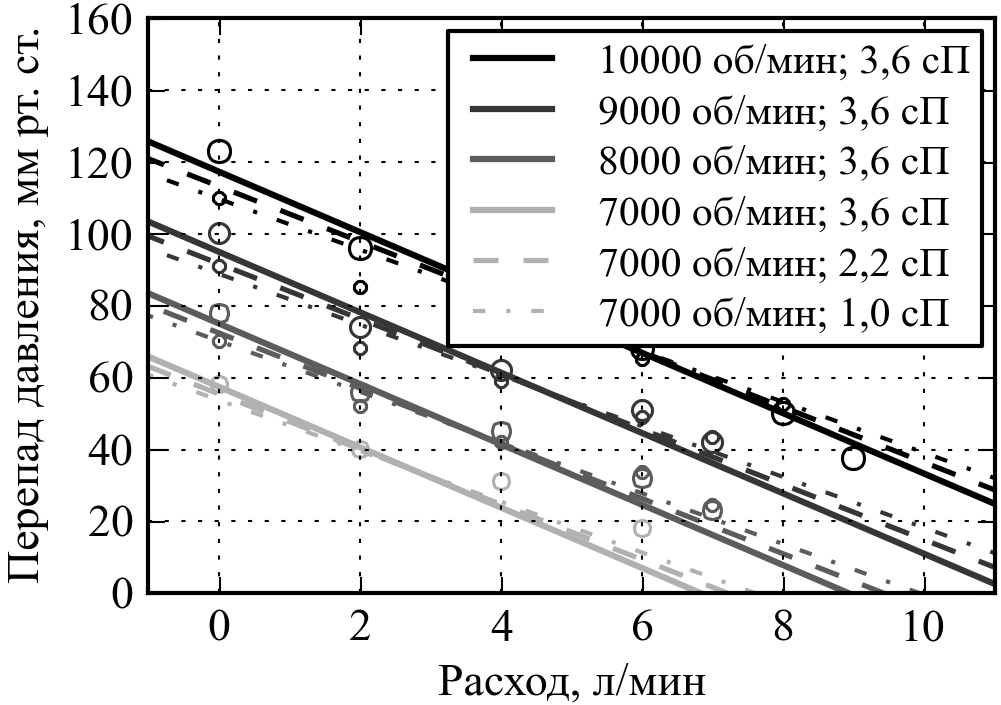
\includegraphics [scale=0.99] {../images/static_model_initial_abs} \\ а)}
  \end{minipage}
  \hfill
  \begin{minipage}[ht]{0.48\linewidth}
    \center{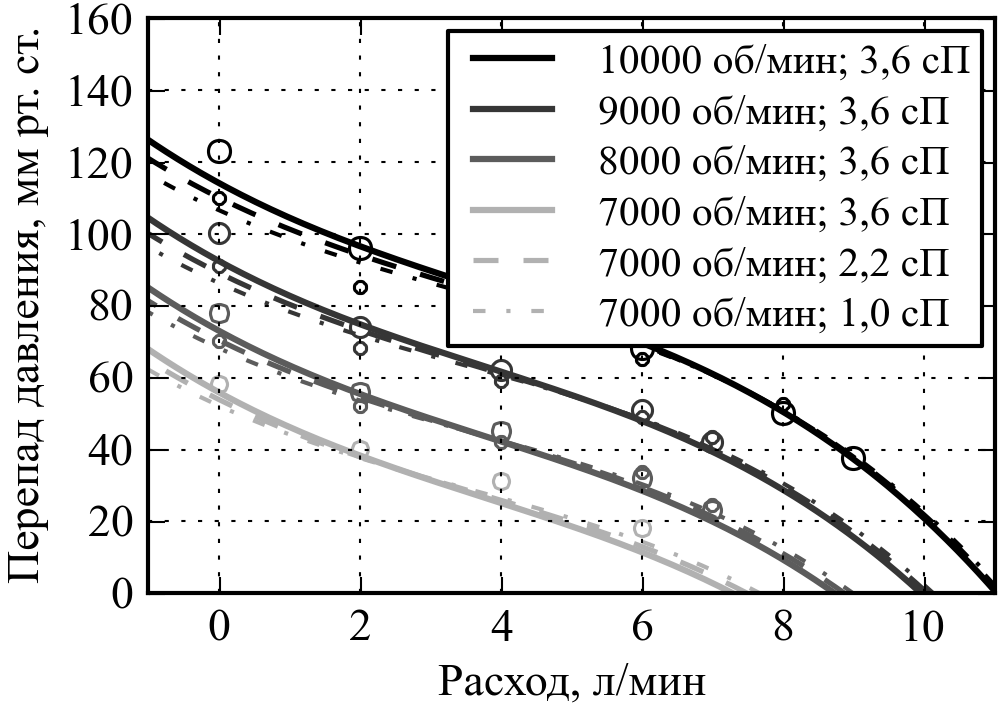
\includegraphics [scale=0.99] {../images/static_model_updated_abs} \\ б)}
  \end{minipage}
  \caption{Расходно-напорные характеристики роторного насоса крови, описываемые уравнением 1 (а) и уравнением 2 (б)}
  \label{img:pump_model_development}  
\end{figure}

После этого к уравнению \eqref{eq:first_step_pump_model} были добавлены члены $Q\omega^2$ и $Q^2 \omega$, а также поправочный коэффициент $g = g_1\mu +g_2$, что позволило увеличить коэффициент детерминации до 0,9987, достичь соответствия моделируемых и экспериментальных РНХ и завершить работу алгоритма.  

Разработанная с использованием алгоритма идентификации математическая модель записывается в следующем виде: 

\begin{multline}
 L\frac{dQ}{dt} = (a_1\mu+a_2)Q + (b_1\mu+b_2)Q^2 + (c_1\mu+c_2)Q^3 + (d_1\mu+d_2)\omega^2 + \\+ (e_1\mu+e_2)Q\omega^2 + (f_1\mu+f_2)Q^2\omega + g_1\mu+g_2 - H.
\label{eq:final_pump_model}
\end{multline}

Поскольку состояние РНК описывается единственной переменной $Q$, то фазовое пространство уравнения \eqref{eq:final_pump_model} одномерно и представлено вещественной прямой $0Q$. Поэтому для наглядности будем изображать эволюцию уравнения \eqref{eq:final_pump_model}, откладывая по оси абсцисс время $t$, по оси ординат -- фазовую переменную $Q$:

\begin{figure}[ht] 
  \center
  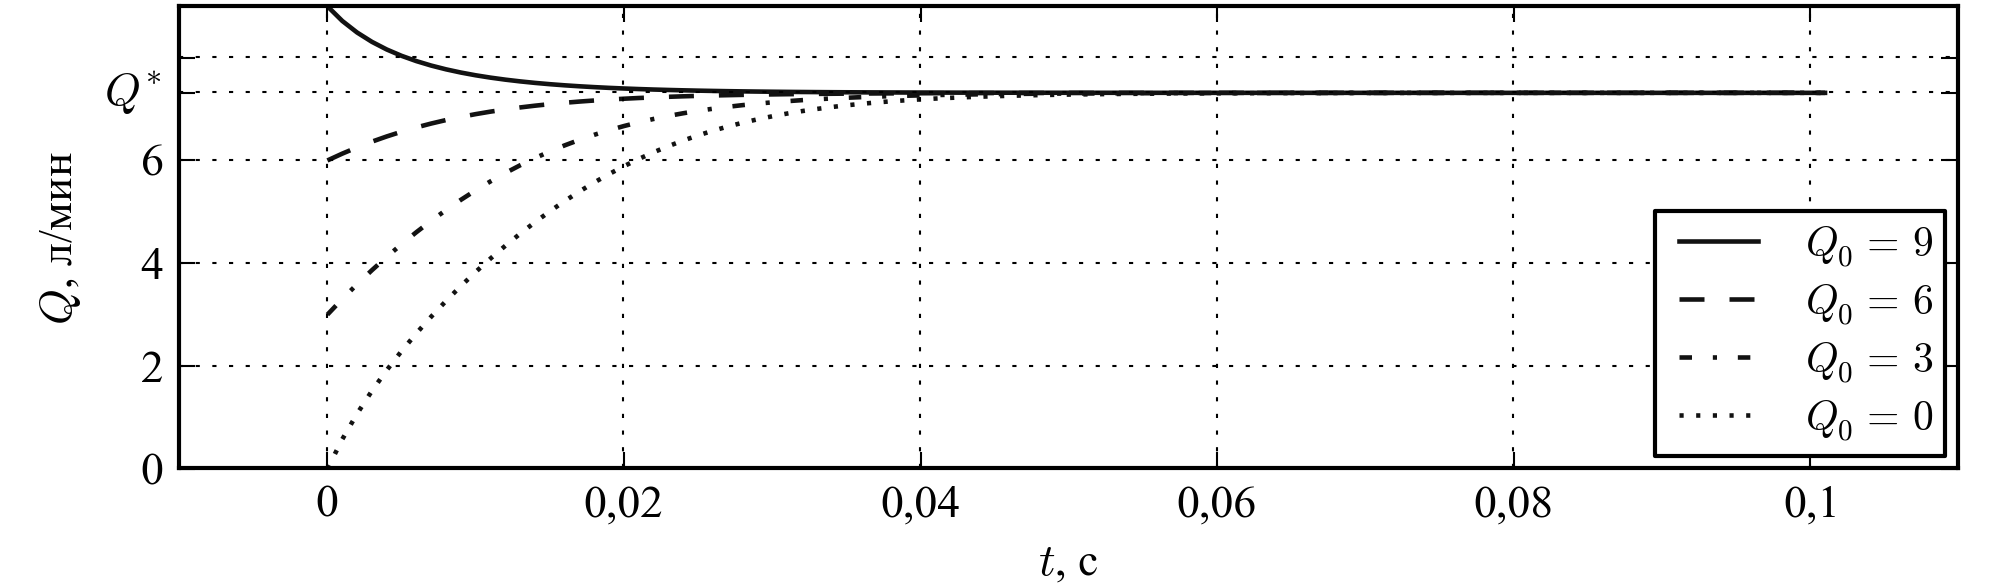
\includegraphics [scale=1.0] {../images/dynamic_model_solution_zero_abs}
  \caption{Зависимость $Q$ от времени при различных начальных условиях}
  \label{img:final_pump_model_solution_zero}  
\end{figure}

На рисунке \ref{img:final_pump_model_solution_zero} представлено изменение $Q$ от времени при фиксированных параметрах $\mu = $ 3,6 сП, $\omega =$ 8000 об/мин и $H = $ 20 мм рт. ст. Видно, что с течением времени значения переменной $Q$ стремятся к некоторому особому значению $Q^*$. При этом значения достаточно быстро выходят на $Q^*$. 

Найдем особые точки уравнения \eqref{eq:final_pump_model}, приравняв левую часть уравнения \eqref{eq:final_pump_model} к нулю:

\begin{multline}
(a_1\mu+a_2)Q + (b_1\mu+b_2)Q^2 + (c_1\mu+c_2)Q^3 + (d_1\mu+d_2)\omega^2 + \\+ (e_1\mu+e_2)Q\omega^2 + (f_1\mu+f_2)Q^2\omega + g_1\mu+g_2 - H = 0.
\label{eq:final_pump_model_zero}
\end{multline}

Уравнение \eqref{eq:final_pump_model_zero} решено с использованием формулы Кардано для нахождения корней $x_1$, $x_2$ и $x_3$ уравнения вида $ax^3 + bx^2 + cx + d = 0$:

\begin{equation}
x_1 = -\frac{b}{3a} + \alpha + \beta, \quad x_{2, 3} = -\frac{b}{3a}  - \frac{(\alpha + \beta)}{2} \pm \frac{i(\alpha - \beta)}{2}\sqrt{3},
\label{eq:cardano_1}
\end{equation}

где 

\begin{equation}
\alpha = \sqrt[3]{-\frac{q}{2} + \sqrt{R}}, \quad \beta = \sqrt[3]{-\frac{q}{2} - \sqrt{R}},
\label{eq:cardano_2}
\end{equation}

\begin{equation}
R = \left(\frac{p}{3}\right)^3 + \left( \frac{q}{2} \right)^2,
\label{eq:cardano_3}
\end{equation}

\begin{equation}
p = \frac{3ac - b^2}{3a^2}, \quad q = \frac{2b^3 - 9abc + 27a^2d}{27a^3}.
\label{eq:cardano_extension}
\end{equation}

Для уравнения \eqref{eq:final_pump_model_zero} $R > 0$, таким образом, уравнение \eqref{eq:final_pump_model_zero} имеет один вещественный корень и два сопряженных комплексных корня, следовательно, при всех физически реализуемых $\mu$, $\omega$ и $H$ особая точка уравнения \eqref{eq:final_pump_model} единственна.% Система для 

%При определенных значениях $\omega$ и $H$ были получены решения, представленные на рисунке \ref{img:final_pump_model_solution}, где маркерами отмечены значения, которые получены в результате численного решения уравнения \eqref{eq:final_pump_model} при $LdQ/dt$ равном нулю с использованием функции \href{https://docs.scipy.org/doc/scipy-0.14.0/reference/generated/scipy.optimize.fsolve.html}{fsolve} из программной библиотеки SciPy.

%\begin{figure}[ht] 
%  \center
%  \includegraphics [scale=1.0] {../images/c2_dynamic_model_solution_abs}
 % \caption{Решение уравнения \eqref{eq:final_pump_model_discret} при различных параметрах $\omega$ и $H$} 
 % \label{img:final_pump_model_solution}  
%\end{figure}

% Решение кубического уравнения, полученного из уравнения \eqref{eq:final_pump_model} посредством приравнивания левой части $LdQ/dt$ к нулю, при определенных значениях $\omega$ и $H$, представлено на рисунке \ref{img:final_pump_model_solution_roots}.



Расходно-напорные характеристики РНК, описываемые разработанной математической моделью идентификации, представлены на рисунке \ref{img:final_pump_model}.

% Разработанная математическая модель идентификации позволяет описать расходно-напорные характеристики, представленные на рисунке \ref{img:final_pump_model}.

\begin{figure}[ht] 
  \center
  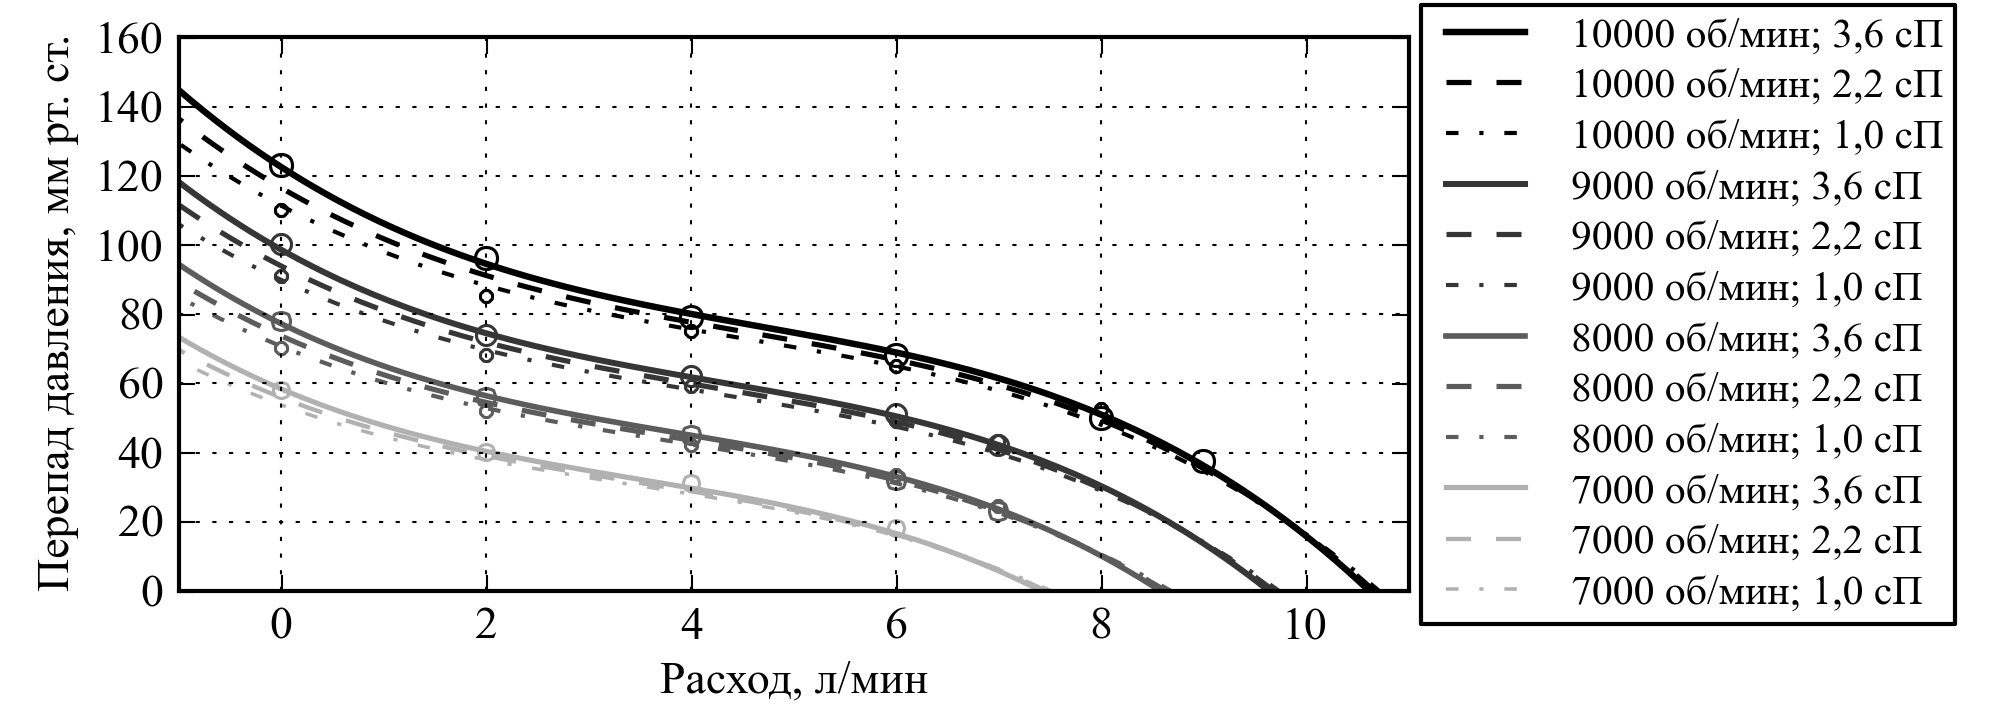
\includegraphics [scale=1.0] {../images/static_model_final_abs}
  \caption{Расходно-напорные характеристики роторного насоса крови, описываемые уравнением \eqref{eq:final_pump_model}} 
  \label{img:final_pump_model}  
\end{figure}

В рамках данного исследования на основе известных математических моделей реализована математическая модель сердечно-сосудистой системы с учетом имплантации роторного насоса крови, которая составлена из математических моделей сердца [11] и системы кровообращения [12] и описывает гемодинамику в сердечно-сосудистой системе с сердечной недостаточностью -- рисунок \ref{img:cvs_hemodynamics}.

\begin{figure}[ht] 
  \center
  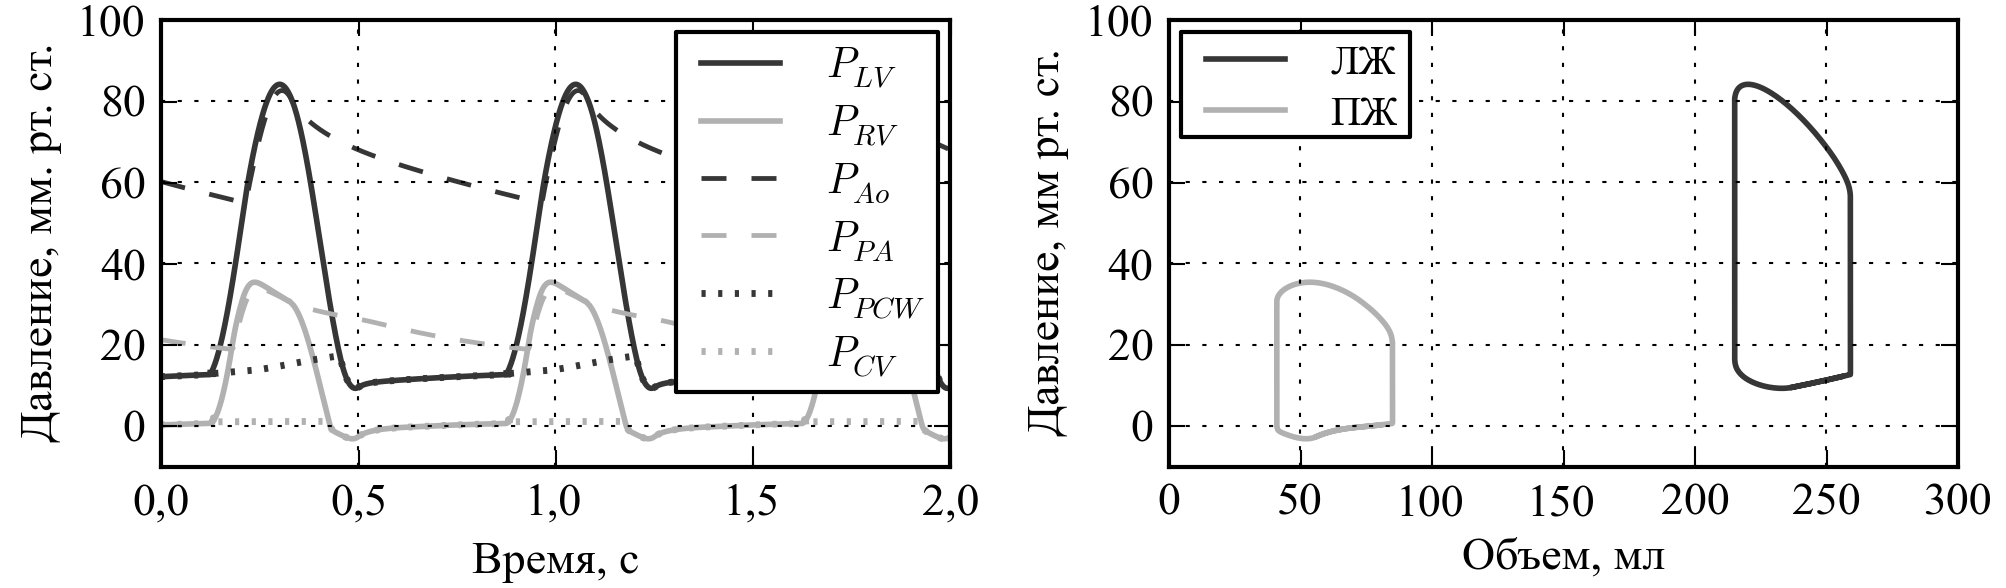
\includegraphics [scale=1.0] {../images/cvs_hemodynamics_abs} 
  \caption{Гемодинамика в сердечно-сосудистой системе для случая сердечной недостаточности; $P_{LV}$ -- давление в левом желудочке, $P_{RV}$ -- давление в правом желудочке, $P_{Ao}$ -- давление в аорте, $P_{PA}$ -- давление в легочной артерии, $P_{CV}$ -- центральное венозное давление, $P_{PCW}$ -- давление заклинивания в легочных капиллярах, ЛЖ -- левый желудочек сердца, \\ПЖ -- правый желудочек сердца}
  \label{img:cvs_hemodynamics}
\end{figure}

% -----------------------------------------------------------------------------------------------------------------------------------------------------------------------------------------
% -----------------------------------------------------------------------------------------------------------------------------------------------------------------------------------------

\underline{\textbf{В третьей главе}} проведено исследование взаимодействия имплантируемого роторного насоса крови и сердечно-сосудистой системы методами математического моделирования. 

%В ходе моделирования получены динамические расходно-напорные характеристики насоса, представленные на рисунке \ref{img:full_dynamic_model}. 

%В ходе исследования выявлена нелинейная форма РНХ, которая обусловлена переходными процессами в роторном насосе крови -- рисунок \ref{img:dynamic_model}. Входными данными математической модели являются временные диаграммы перепада давления при двух значениях параметра $\omega$, выходными данными математической модели являются временные диаграммы расхода насоса.

%\begin{figure}[ht] 
%  \center
%  \includegraphics [scale=1.0] {../images/c2_dynamic_model_edit_abs}
%  \caption{Временные диаграммы расхода и перепада давления (слева) и соответствующие расходно-напорные характеристики роторного насоса крови при 7000 об/мин и 9000 об/мин %(справа)} 
%  \label{img:dynamic_model}
%\end{figure}

В ходе исследования получены зависимости, описывающие изменения в гемодинамике сердечно-сосудистой системы при различных скоростях насоса -- рисунок \ref{img:pumping_states_general}. 

\begin{figure}[!ht] 
  \center
  \noindent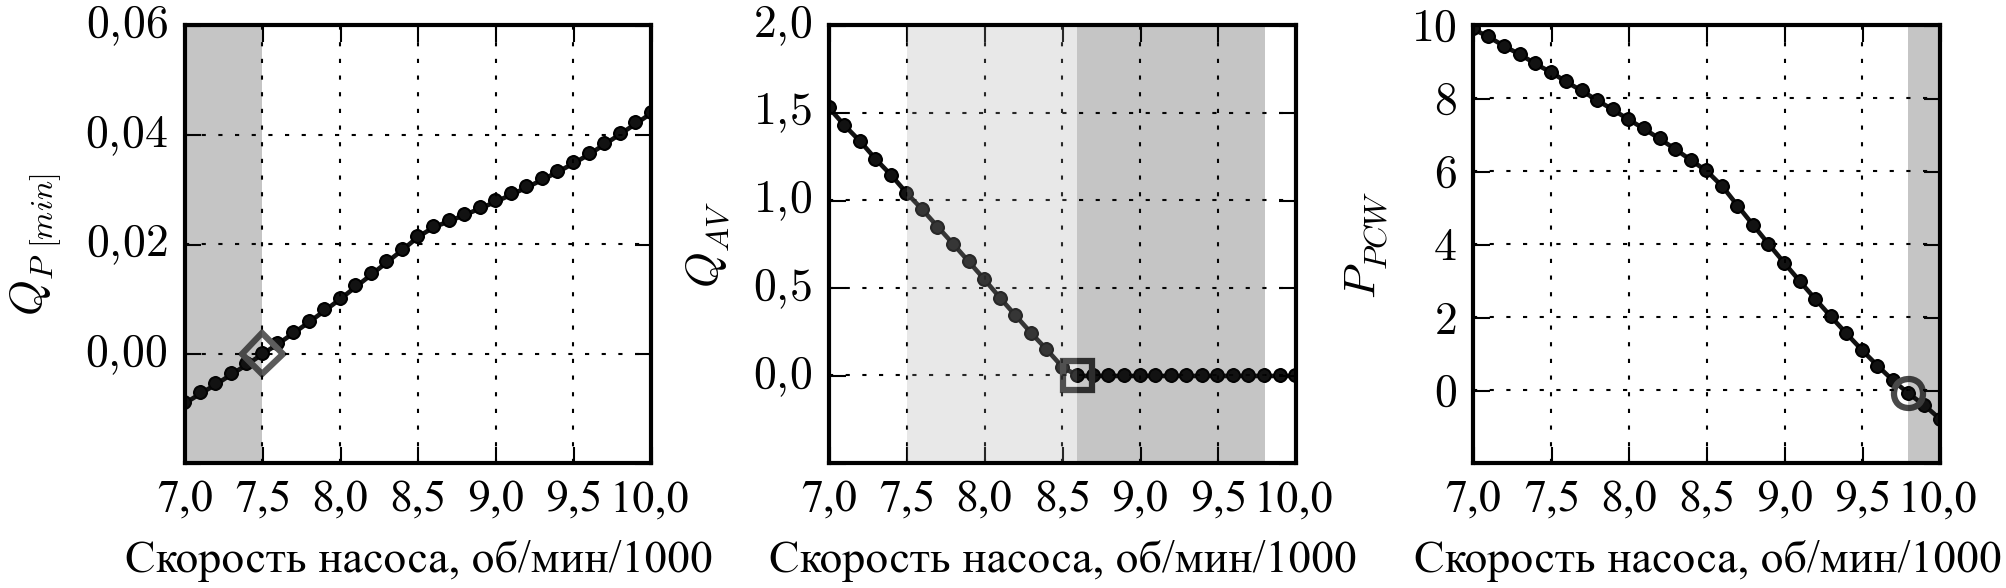
\includegraphics [scale=1.0] {../images/pumping_states_abs}
  \caption{Гемодинамические зависимости, полученные на математической модели сердечно-сосудистой системы; $Q_{P[min]}$ -- минимальный расход насоса (л/с), $Q_{AV}$ -- поток через аортальный клапан (л/мин), $P_{PCW}$ -- давление заклинивания в легочных капиллярах (мм рт. ст.)} 
  \label{img:pumping_states_general}  
\end{figure}

Полученные зависимости позволяют определить следующие режимы работы насоса: обратное течение через насос ($P_{BF}$), частичная разгрузка ($P_{PA}$) и полная разгрузка желудочка сердца ($P_{FA}$), коллапс желудочка сердца ($P_{VC}$). 

Так, режиму обратного течения $P_{BF}$ соответствует диапазон скоростей насоса с отрицательным расходом во время сердечного цикла -- данный диапазон выделен серым цветом на диаграмме $Q_{P[min]}$. Аналогичным образом режимам работы $P_{PA}$ и $P_{FA}$ соответствуют диапазоны скоростей с ненулевым и нулевым потоками через аортальный клапан, которые выделены соответственно светло-серым и серым цветом на диаграмме $Q_{AV}$; режиму коллапса желудочка сердца $P_{VC}$ соответствует диапазон скоростей с отрицательным давлением, который выделен серым цветом на диаграмме $P_{PCW}$.

% Таким образом, на рисунке \ref{img:pumping_states_general} синим цветом на зависимости $Q_{P[min]}$ обозначен диапазон скоростей насоса, которому соответствует режим обратного течения. 

В результате анализа закономерностей взаимодействия имплантируемого роторного насоса крови и сердечно-сосудистой системы на основе модели идентификации разработан метод определения режимов работы насоса. Метод заключается в нахождении производных из модели идентификации, вычислении их значений при различных скоростях насоса и определении тех производных, изменение которых коррелирует с режимами работы насоса. 

Разработанный метод характеризуется точностью определения перехода между режимами работы насоса, которая рассчитывается по следующей формуле:

\begin{equation}
	\label{eq:ps_identification_accuracy}
	\delta(PS) = \left(1 - \frac{\lvert\hskip2pt \omega_t - \omega_m \rvert}{\omega_{max} - \omega_{min}} \right) \cdot 100\%,
\end{equation}

\noindent где $\omega_t$ -- практическое значение скорости насоса, при которой происходит переход между режимами работы, $\omega_m$ -- полученное из метода расчетное значение скорости насоса, при которой происходит переход между режимами работы, $\omega_{max}$ и $\omega_{min}$ -- верхняя и нижняя граница скорости вращения ротора насоса.

Результаты расчета точности при изменении сократимости левого желудочка сердца и частоты сердечных сокращений для трех значений параметра $\mu$ модели идентификации представлены в таблице \ref{tbl:ps_identification_accuracy_model}. %Приведенные значения являются средними при изменении сократимости левого желудочка сердца на $\pm$10\% и частоте сердечных сокращений от 60 до 100 уд/мин с шагом 20 уд/мин.

\begin{table} [htbp]%
    \centering
	\caption{Точность определения переходов между режимами работы насоса ($\delta(PS)$, \%)}%
	\label{tbl:ps_identification_accuracy_model}%
    \renewcommand{\arraystretch}{1.5} 
	\begin{tabular}{@{}@{\extracolsep{22pt}}llll@{}} 
	\toprule
	& $\mu = $ 3,6 сП & $\mu = $ 2,2 сП & $\mu = $ 1,0 сП\\
	\midrule
	$\delta(P_{BF}/P_{PA})$			& 88,7		&	87,5 & 85,4\\
	$\delta(P_{PA}/P_{FA})$				& 98,0		& 97,9	& 97,6\\
	%$\delta(P_{FA}/P_{PVC})$			& 90,6		& 94,5	& 94,4\\
	$\delta(P_{FA}/P_{VC})$		& 82,7		& 83,4	& 82,6\\
    \bottomrule 
	\end{tabular}%
\end{table}

В результате проведенного комплексного исследования разработан способ управления имплантируемым роторным насосом крови, представленный с помощью системы управления скоростью РНК на рисунке \ref{img:control_algorithm}. 

%Управление насосом заключается в регулировании скорости вращения ротора. 

\begin{figure}[ht] 
  \center
  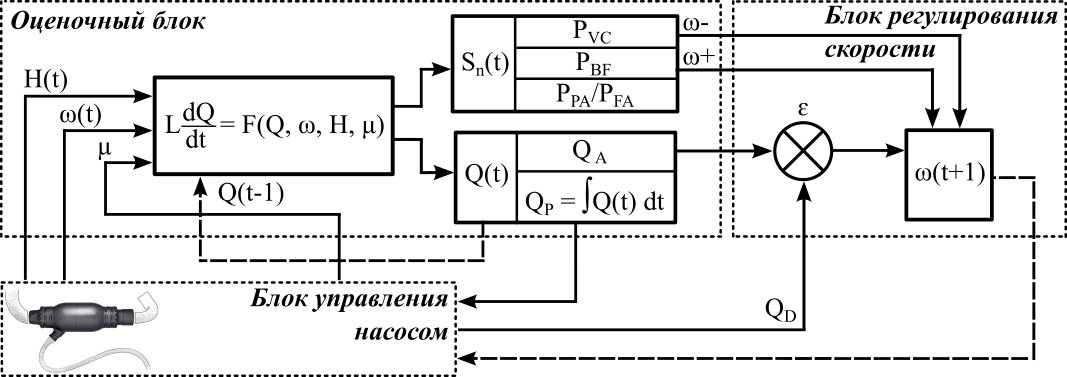
\includegraphics [scale=1.66] {../images/c3_control_algorithm}
  \caption{Обобщенная структура системы управления скоростью роторного насоса крови} 
  \label{img:control_algorithm}  
\end{figure}

В \textit{оценочном блоке} с использованием модели идентификации осуществляется определение режима работы и оценка расхода насоса по данным о перепаде давления в насосе ($H$, мм рт. ст.), который регистрируется в математической модели сердечно-сосудистой системы, скорости вращения ротора ($\omega$, об/мин) и вязкости жидкости ($\mu$, сП), которые задаются в \textit{блоке управления насосом}. 
 
В \textit{блоке регулирования скорости} формируется новое значение скорости вращения ротора $\omega(t+1)$, которое зависит от текущего режима работы насоса и от разности $Q_A$ и $Q_D$, где $Q_A$ -- расход насоса в течение нескольких сердечных циклов и $Q_D$ -- заданный уровень расхода насоса. 

В случае неравенства $Q_A$ и $Q_D$ происходит изменение скорости на 100 об/мин. При выявлении нежелательного режима работы насоса, такого как $P_{VC}$, скорость вращения ротора уменьшается на 500 об/мин независимо от разности $Q_A$ и $Q_D$. % независимо от величины $Q_A$ 

Разработанный способ управления скоростью имплантируемого роторного насоса крови исследован на математической модели сердечно-сосудистой системы при изменении сократимости левого желудочка сердца и частоты сердечных сокращений. Результаты продемонстрировали возможность поддержания заданного уровня расхода насоса и предотвращения следующих нежелательных режимов работы насоса: обратное течение через насос, полная разгрузка желудочка сердца и коллапс желудочка сердца. 

В результате анализа разработанного способа управления предложены следующие критерии оценки эффективности идентификации: точность оценки расхода насоса и точность определения перехода между режимами работы насоса.

% -----------------------------------------------------------------------------------------------------------------------------------------------------------------------------------------
% -----------------------------------------------------------------------------------------------------------------------------------------------------------------------------------------

\underline{\textbf{В четвертой главе}} проведено исследование взаимодействия насоса и сердечно-сосудистой системы с использованием экспериментальных данных для имплантируемых роторных насосов крови Спутник.
%\paragraph{Протокол исследования.}

Фотографии насосов -- далее Спутник 1 и Спутник 2 -- представлены на рисунке \ref{img:sputnik_pumps}. % 

% \begin{figure}[ht]
%   \begin{minipage}[ht]{0.42\linewidth}
%     \center{\includegraphics [scale=0.47] {../images/s1_pump_abs} \\ а)}
%   \end{minipage} 
%   \hfill
%   \begin{minipage}[ht]{0.54\linewidth}
%     \center{\includegraphics [scale=0.47] {../images/s2_pump_abs} \\ б)}
%   \end{minipage}
%   \caption{Имплантируемые роторные насосы крови Спутник первого (а) и второго поколений (б)}
%   \label{img:sputnik_pumps}  
% \end{figure}

\begin{figure}[ht]
  \begin{minipage}[ht]{0.48\linewidth}
    \center{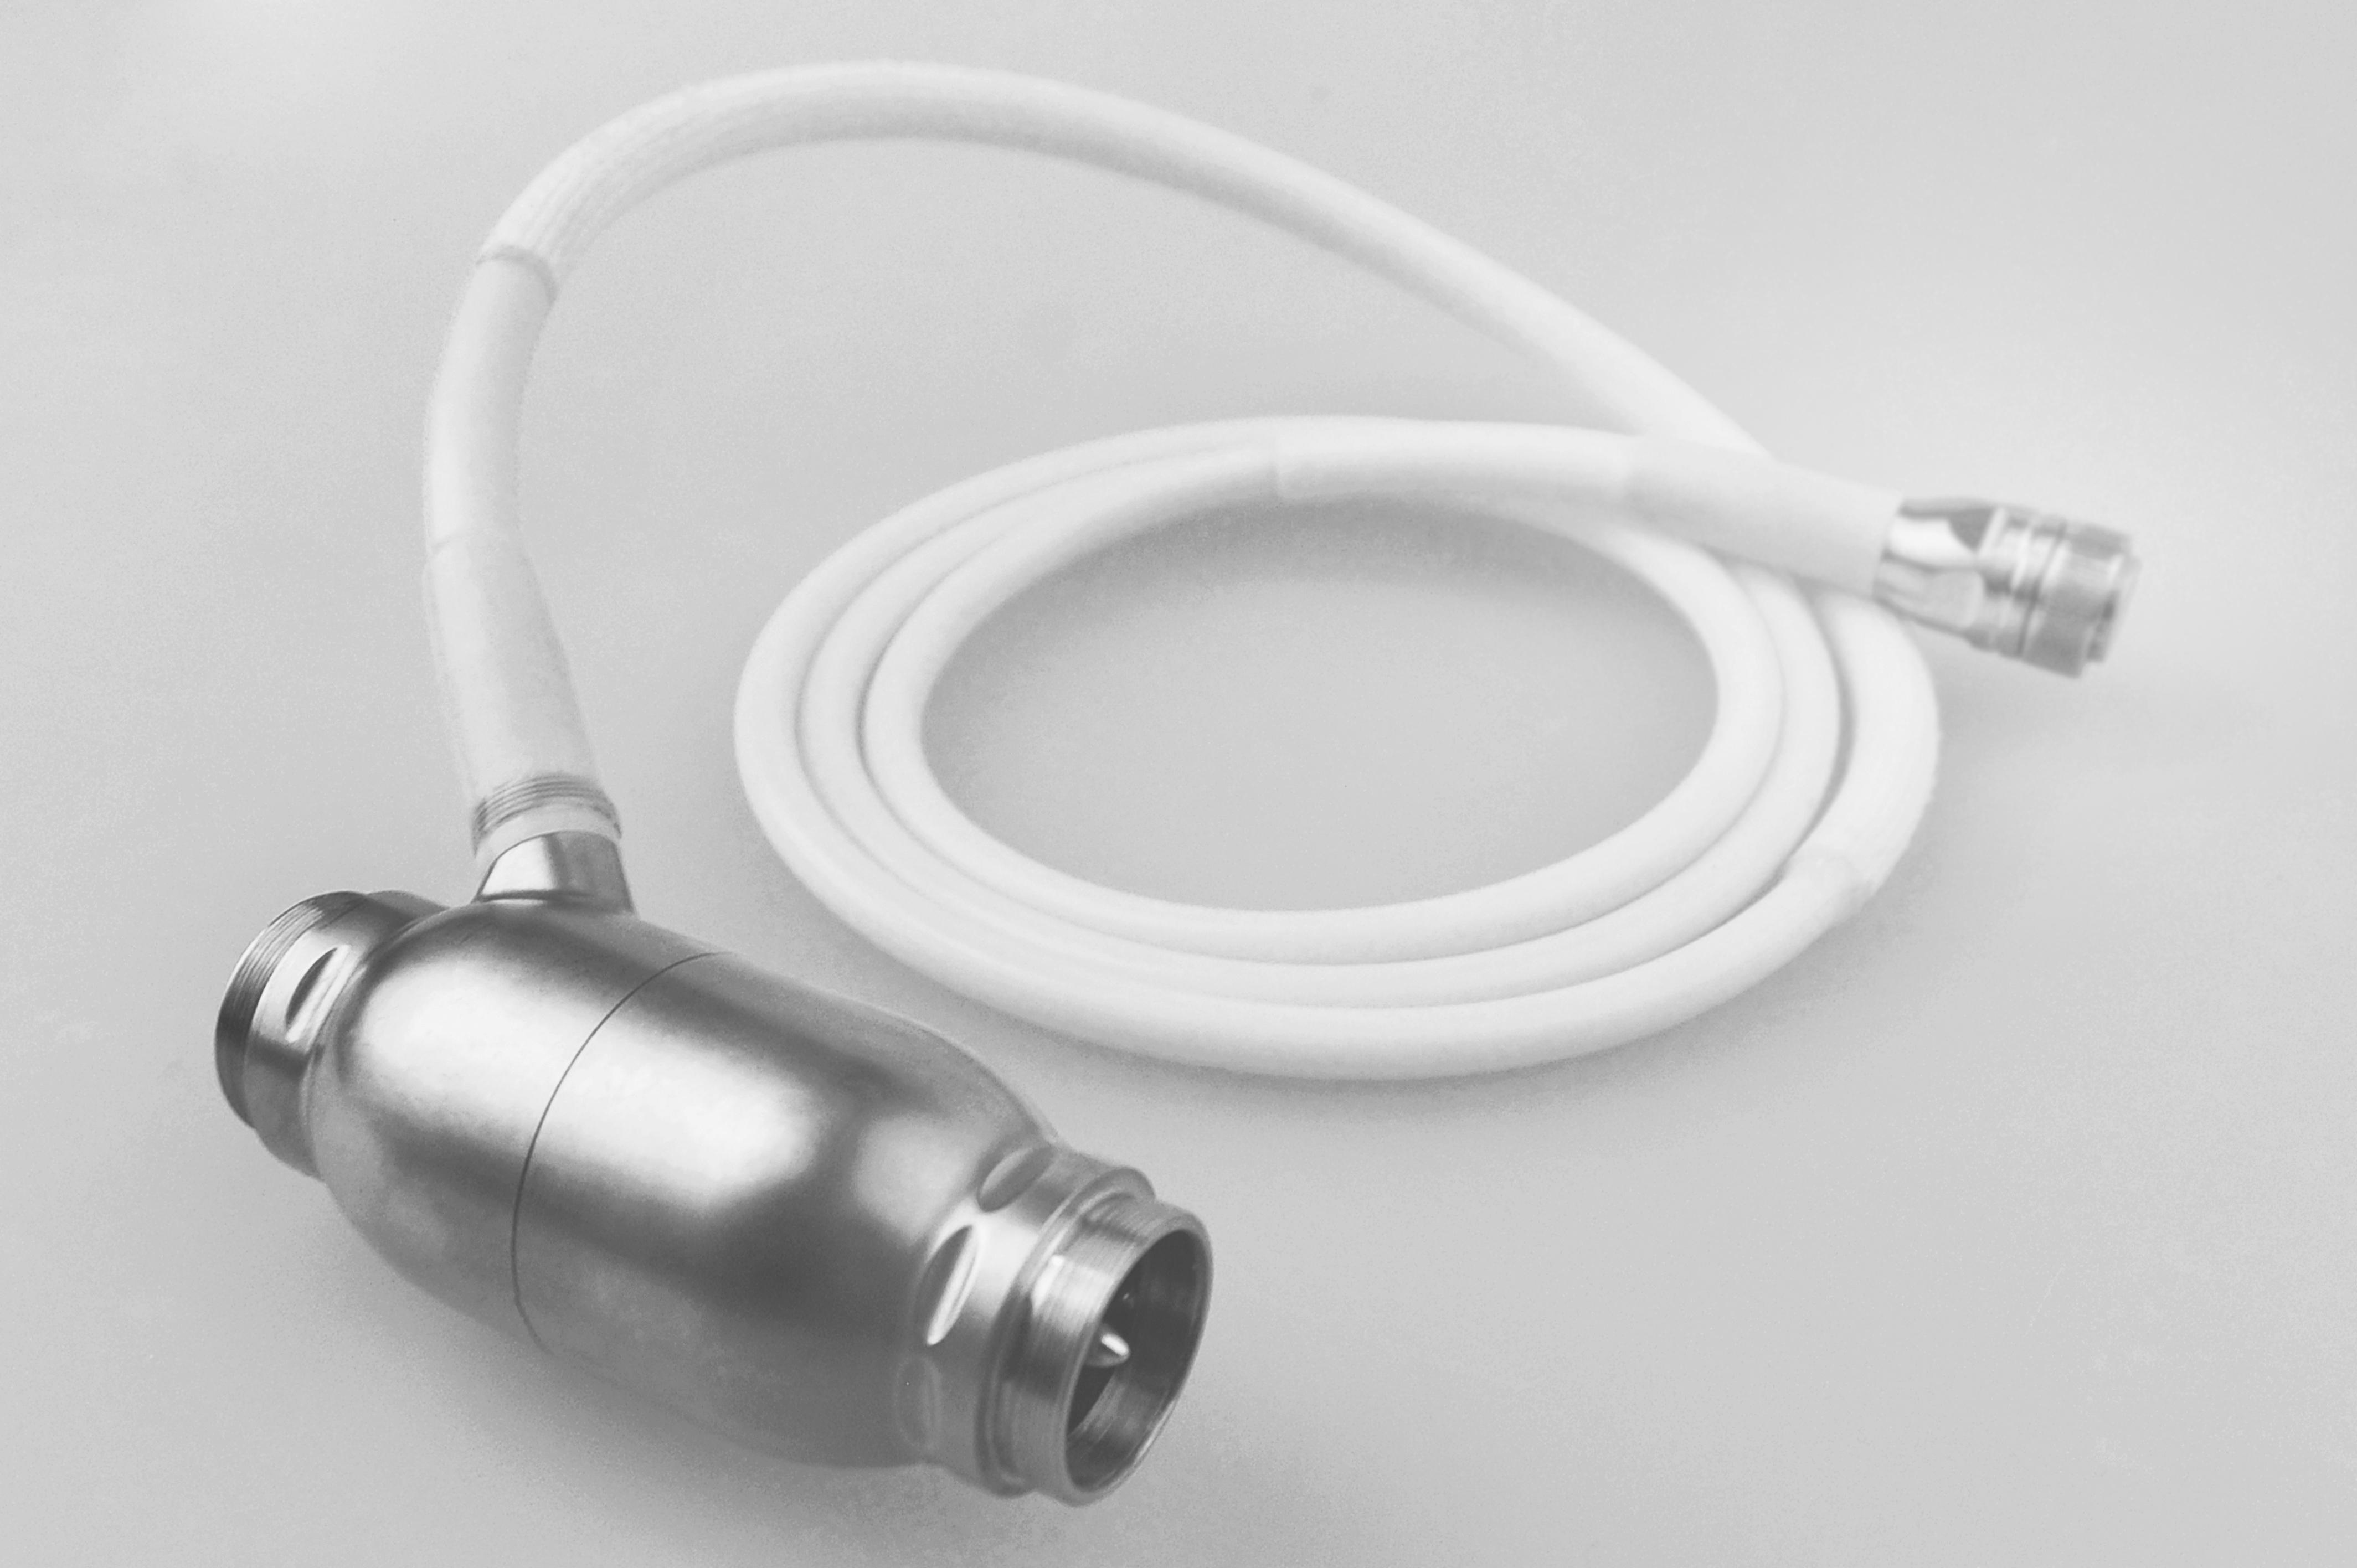
\includegraphics [scale=0.225] {../images/s1_abs} \\ а)}
  \end{minipage}
  \hfill
  \begin{minipage}[ht]{0.48\linewidth}
    \center{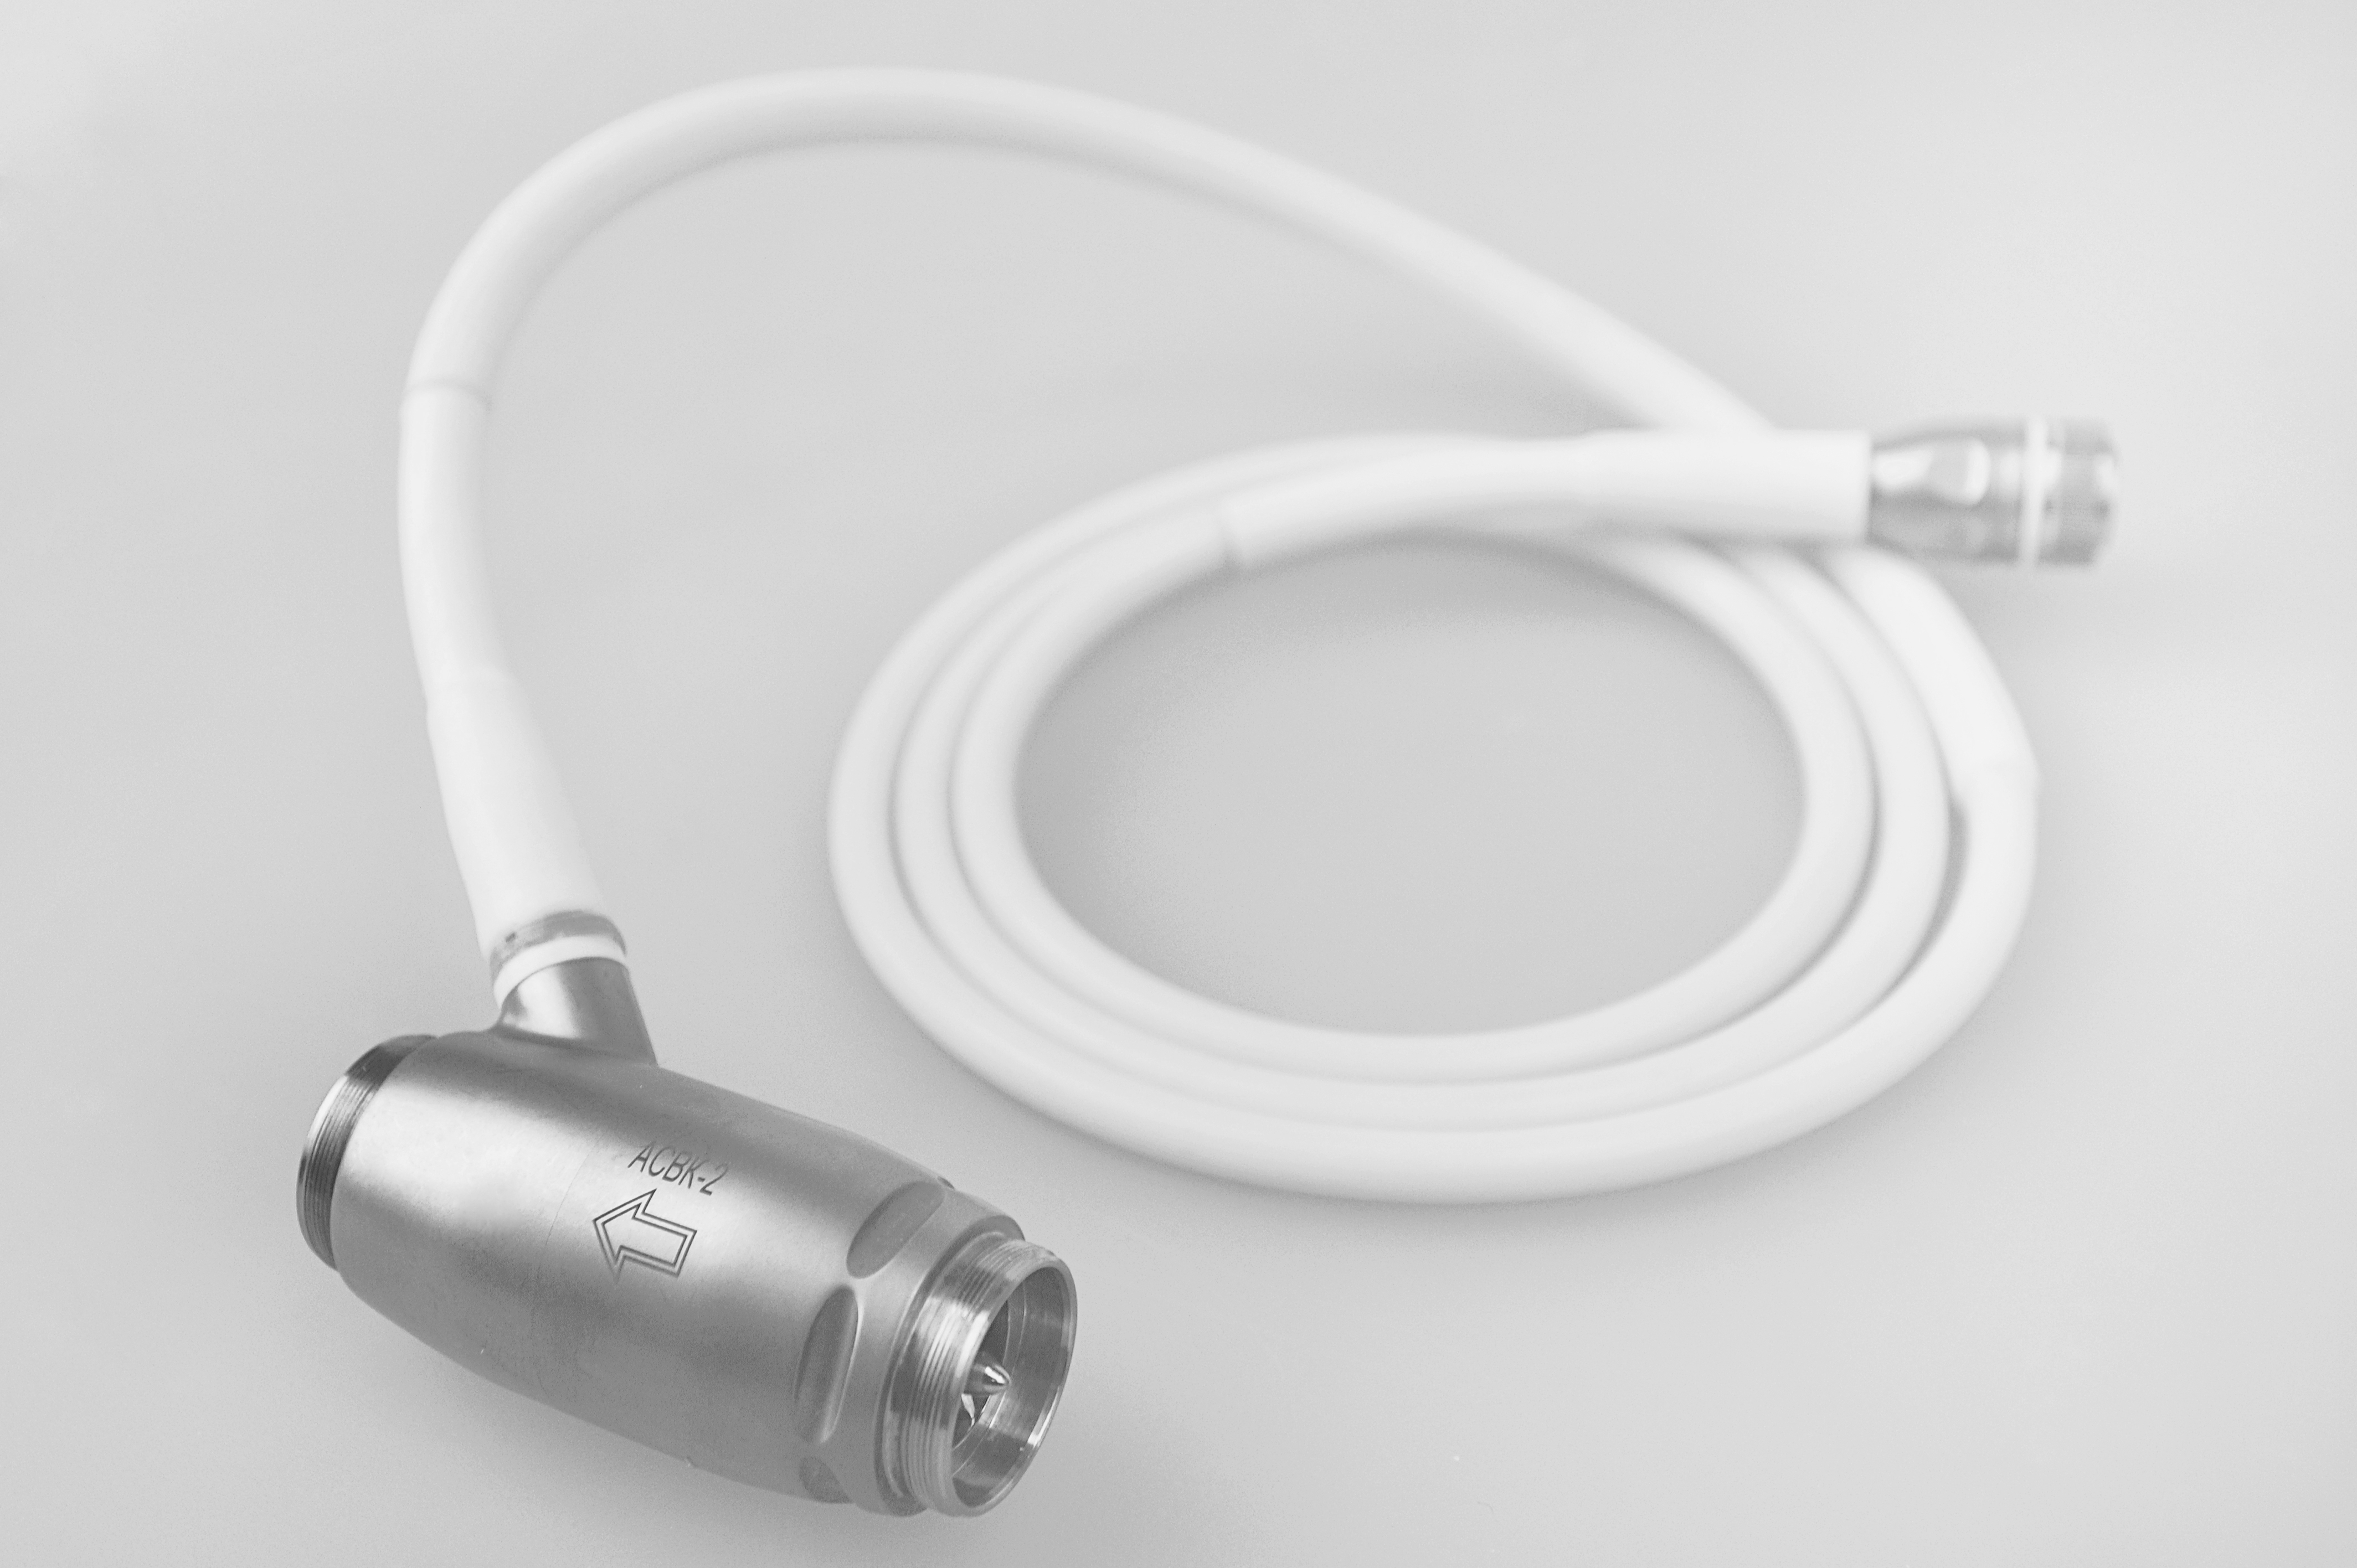
\includegraphics [scale=0.225] {../images/s2_abs} \\ б)}
  \end{minipage}
  \caption{Имплантируемые роторные насосы крови Спутник первого (а) \\и второго поколений (б)}
  \label{img:sputnik_pumps}  
\end{figure}

% \begin{figure}[ht]
%   \center{\includegraphics [scale=0.50] {../images/c5_Sputniks}}
% %   \begin{minipage}[ht]{0.49\linewidth}
% %     \center{\includegraphics [scale=1.0] {../images/c5_sputnik_1} \\ а)}
% %   \end{minipage}
% %   \hfill
% %   \begin{minipage}[ht]{0.49\linewidth}
% %     \center{\includegraphics [scale=0.93] {../images/c5_sputnik_2} \\ б)}
% %   \end{minipage}
%   \caption{Имплантируемые роторные насосы крови Спутник первого (слева) и второго поколений (справа)}
%   \label{img:sputnik_pumps}  
% \end{figure}

Эксперимент проведен в испытательном гидродинамическом стенде, расположенном в Институте Гельмгольца по биомедицинской инженерии (г. Ахен, Германия) [13]. Схема гидродинамического стенда представлена на рисунке \ref{img:mcl}. Система управления стендом с помощью специальных приводных механизмов формировала давления в камерах $C_{in}$ и $C_{out}$, что позволяло создать перепад давления в системе аналогично сердечно-сосудистой системе.

\begin{figure}[!ht] 
  \center
  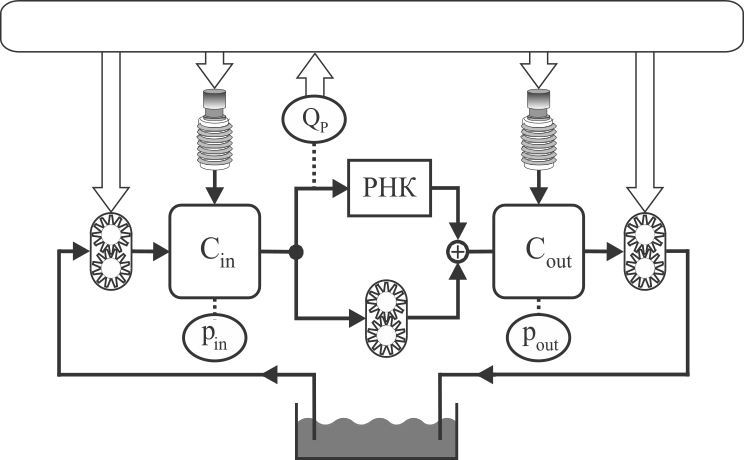
\includegraphics [scale=1.8] {../images/mcl_scheme_abs}
\begin{tikzpicture}[node distance=1cm, auto, overlay]  
\draw (-5.75, 6.59) node {\small \scalebox{1.075}{Система управления испытательным стендом}}; %  \\ $\delta(PS) \geq 85\%$
\end{tikzpicture} 
  \caption{Схема испытательного гидродинамического стенда} 
  \label{img:mcl}  
\end{figure}

Вязкость жидкости в контуре гидродинамического стенда равнялась 2,5 сП, частота сердечных сокращений -- 80 уд/мин, скорость вращения ротора каждого насоса изменялась в диапазоне от 5 до 10 тысяч об/мин с шагом 200 об/мин. В стенде последовательно воспроизводились два состояния сердечно-сосудистой системы, соответствующие различным степеням сердечной недостаточности. Данные состояния были воспроизведены посредством задания физиологического параметра contractilityFactor (cF) равным 0,5 и 0,25, где cF равное 1 соответствует нормальной функции сердца.

%Скорость вращения ротора насоса изменялась в диапазоне от 5000 до 10000 об/мин с шагом 200 об/мин. На каждом шаге в течение примерно 30 секунд записывались данные о расходе насоса, скорости вращения ротора, давлении на входе и выходе насоса и потоке через аортальный клапан.

%\paragraph{Исследование алгоритма идентификации.}

% проведено исследование алгоритма идентификации с использованием результатов, полученных в ходе эксперимента. 

В рамках данного исследования были выбраны следующие критерии оценки эффективности идентификации: точность оценки расхода насоса и точность определения перехода между режимами работы насоса. Для выбранных критериев заданы следующие пороговые величины: средняя точность оценки расхода $\geq$ 90 \%, средняя точность определения перехода $\geq$ 80 \%. 

Точность оценки расхода насоса для каждой скорости вращения ротора рассчитывалась по следующей формуле:

\begin{equation}
	\delta(Q) = \left( 1 - (Q_M - Q_E)/Q_M \right) \cdot 100 \%,
\end{equation}

\noindent где $Q_M$ -- расход насоса, измеренный датчиком, $Q_E$ -- расход насоса, вычисленный с помощью математической модели. %Точность определения переходов между режимами работы насоса рассчитывалась согласно \eqref{eq:ps_identification_accuracy}. 

Точность определения перехода между режимами работы насоса рассчитывалась по формуле \eqref{eq:ps_identification_accuracy}. 

В ходе анализа экспериментальных данных режим коллапса желудочка сердца $P_{VC}$ был определен как отрицательное конечно-диастолическое давление в желудочке сердца. 

Первоначально для описания имплантируемых роторных насосов крови Спутник использована математическая модель идентификации, представленная уравнением \eqref{eq:final_pump_model}. Коэффициенты данной модели определены для состояния cF 0,5 с использованием разработанной процедуры оптимизации на основе алгоритма дифференциальной эволюции [14]. Оценка соответствия критериям эффективности идентификации выполнена посредством вычисления средней точности оценки расхода и точности определения переходов между режимами работы насоса для двух состояний сердечно-сосудистой системы с различными параметрами cF. 

Установлено, что средняя точность оценки расхода с использованием разработанной модели идентификации для Спутник 1 составляет 97,6\%, для Спутник 2 -- 82,5\%, точность определения перехода $P_{FA}/P_{VC}$ составляет менее 75\% для обоих насосов. 

Таким образом, разработанная модель идентификации не позволяет обеспечить соответствие заданным пороговым величинам для критериев оценки эффективности идентификации.

%С целью обеспечения соответствия заданным пороговым величинам использован разработанный алгоритм идентификации. При этом построение математической модели осуществлялось в соответствии с предложенными критериями для оценки эффективности идентификации. 
%Измененная блок-схема алгоритма идентификации представлена на рисунке \ref{img:flowchart_upd}.

Данная проблема решена посредством построения математических моделей с использованием алгоритма структурно-параметрической идентификации. В качестве исходного уравнения $y_i$ в алгоритме выбрано уравнение \eqref{eq:initial_eq}, заданный список одночленов $kx_j$ заменен на член $k\omega^xH^yQ^z$, где $k$ -- коэффициент, $x$, $y$ и $z$ $\in [-2 .. 4].$ % целые числа в диапазоне от -2 до 4. % в соответствии с критериями оценки эффективности идентификации

Построение математических моделей осуществлялось в соответствии с выбранными критериями оценки эффективности идентификации. Коэффициенты уравнений вида $y_i + k\omega^xH^yQ^z$ также определялись для состояния cF 0,5 с использованием разработанной процедуры оптимизации. В случае соответствия полученного уравнения только одному из критериев оценки эффективности идентификации запускался вложенный цикл алгоритма с добавлением членов $k\omega^xH^yQ^z$, определением коэффициентов уравнений и проверкой на соответствие критериям.

%В результате исследования были построены модели идентификации имплантируемых роторных насосов крови в соответствии с критериями для оценки эффективности идентификации.

% \begin{figure}[ht]
% \centering
% \begin{tikzpicture}[node distance=1cm, auto]  
% % \tikzset{
% %     mynode/.style={rectangle,rounded corners,draw=black, top color=white, bottom color=yellow!50,very thick, inner sep=1em, minimum size=3em, text centered},
% %     myarrow/.style={draw},
% % }
% 
% % \node[mynode] (top) {Государственная власть};  
% % \node[mynode, below=2cm of top] (center) {Судебная};
% % \node[mynode, left=of center] (left) {Законодательная};
% % \node[mynode, right=of center] (right) {Исполнительная};
% % 
% % \draw[myarrow] (top.south) -- (center.north);   
% % \draw[myarrow] (top.south) -- ++(0,-1) -|  (left.north);        
% % \draw[myarrow] (top.south) -- ++(0,-1) -|  (right.north);
% 
% \tikzstyle{startstop} = [rectangle, rounded corners, minimum width=1cm, minimum height=0.8cm,text centered, draw=black, fill=gray!10]
% \tikzstyle{io} = [trapezium, trapezium left angle=70, trapezium right angle=110, minimum width=1cm, minimum height=0.8cm, text centered, draw=black, fill=gray!10]
% \tikzstyle{process} = [rectangle, minimum width=1cm, minimum height=0.8cm, text centered, draw=black, fill=blue!30]
% \tikzstyle{decision} = [diamond, minimum width=3.0cm, minimum height=1.4cm, text centered, draw=black, fill=gray!10]
% \tikzstyle{arrow} = [thick,->,>=stealth]
% 
% \node (start) [startstop] {\small \parbox{5.7cm}{Задание исходного выражения и пороговых величин для критериев оценки эффективности}};
% \node (in1) [io, below of=start, yshift=-1.0cm] {\small \parbox{5.2cm}{Прибавление к исходному выражению члена $k\omega^xH^yQ^z$}};
% \node (pro1) [process, below of=in1, yshift=-1.1cm] {\small \parbox{6.4cm}{Оптимизация уравнения для cF 0,5.\\Проверка на соответствие пороговым величинам для cF 0,5 и cF 0,25}};
% \node (dec1) [decision, below of=pro1, yshift=-1.2cm] {};% {\footnotesize\bf \parbox{1.5cm}{Соответствие \\ критериям}};
% \node (out2a) [process, right of=dec1, xshift=5.2cm, minimum width=1.0cm, fill=yellow!40] {\small \parbox{5.0cm}{Задание \\ $LdQ/dt=\ldots + k\omega^xH^yQ^z$ исходным выражением}};
% \node (out2b) [io, left of=dec1, xshift=-3.5cm, minimum width=1.0cm, fill=red!40] {\small \parbox{2.0cm}{Исключение данного\\ уравнения}};
% \node (stop) [startstop, below of=dec1, yshift=-0.5cm, fill=green!40, yshift=-0.1cm] {\small Окончательное уравнение};
% 
% \draw [arrow] (start) -- (in1);
% \draw [arrow] (in1) -- (pro1);
% \draw [arrow] (pro1) -- (dec1);
% \draw [arrow] (dec1) -- (out2a);
% \draw [arrow] (dec1) -- (out2b);
% \draw [arrow] (dec1) -- (stop);
% \draw [arrow] (out2a) |- ($(in1.east)+(0,-0.1)$);
% \draw [arrow] (out2b) |- (in1.west);%($(start.south)!0.16!(pro1.north)$);
% % $(processing.south)-(0,0.5)$
% \draw [arrow] (dec1) -- node[anchor=south] {\footnotesize\it частично} (out2a);
% \draw [arrow] (dec1) -- node[anchor=north] {\footnotesize\it нет} (out2b);
% \draw [arrow] (dec1) -- node[anchor=west] {\footnotesize\it да} (stop);
% 
% \end{tikzpicture} 
% \caption{Блок-схема алгоритма идентификации роторного насоса крови} 
% \label{img:flowchart_upd}  
% \end{figure}

% \begin{enumerate}
%  \begin{itemize}
%   \item если ни один из критериев не выполнялся, то данное уравнения исключалась из рассмотрения,
%   \item если выполнялся хотя бы один из критериев, то уравнение вида $LdQ/dt = \ldots + \omega^xH^yQ^z$ задавалось в качестве исходного выражения и алгоритм повторялся с шага 1,
%   \item если все критерии оценки выполнялись, то процесс разработки заканчивался.
%  \end{itemize}
% \end{enumerate}

В результате применения алгоритма идентификации были построены математические модели, которые обеспечивают соответствие заданным пороговым величинам для критериев оценки эффективности идентификации. 

Математическая модель насоса Спутник 1 описывается следующим уравнением:

\begin{equation}
	\label{eq:sputnik_1_eq}
	L_1\frac{dQ}{dt} = a_1Q + b_1\omega^2 + c_1H + d_1HQ + e_1\omega^{-1} H^2 Q.
\end{equation}

Математическая модель насоса Спутник 2 описывается следующим уравнением:

\begin{equation}
	\label{eq:sputnik_2_eq}
	L_2\frac{dQ}{dt} = a_2Q + b_2\omega^2 + c_2H + d_2HQ^3 + e_2\omega^{-1}Q.
\end{equation}

%Точность определения переходов между режимами работы насоса и 

Средняя точность оценки расхода насоса и точность определения переходов между режимами работы, рассчитанные с помощью экспериментальных данных для Спутник 1 и Спутник 2, представлены в таблице \ref{tbl:sputnik_ps_identification_accuracy}. 

\begin{table} [htbp]%
    \centering
	\caption{Средняя точность оценки расхода насоса ($\delta(Q_{mean})$, \%) и точность определения перехода между режимами работы насоса ($\delta(PS)$, \%)\vskip5pt}%
	\label{tbl:sputnik_ps_identification_accuracy}% label всегда желательно идти после caption
    \renewcommand{\arraystretch}{1.5} 
	\begin{tabular}{@{}@{\extracolsep{22pt}}lllll@{}} 
	\toprule
	& \multicolumn{2}{c}{Спутник 1} & \multicolumn{2}{c}{Спутник 2} \\
	\midrule
				&	cF 0,5	& cF 0,25 &	cF 0,5 & cF 0,25\\
	\midrule
	$\delta(Q_{mean})$			& 	93,7			&	93,6			& 90,1			& 94,6\\
	\midrule
	$\delta(P_{BF}/P_{PA})$	& 91,7			&	91,7			& 100,0		& 100,0\\
	$\delta(P_{PA}/P_{FA})$		& 100,0		&	100,0		& 100,0		& 100,0\\
	$\delta(P_{FA}/P_{VC})$	& 	100,0		&	100,0		& 91,7			& 91,7\\
	\bottomrule
	\end{tabular}%
\end{table}

%Точность определения переходов между режимами работы насоса также была вычислена в ходе исследований разработанных моделей идентификации на модели сердечно-сосудистой системы. В этом случае точность определения перехода $P_{BF}/P_{PA}$ составила не менее 92\%, перехода $P_{PA}/P_{FA}$ -- 100\%.
% и приведена в столбце <<Модель>> таблицы \ref{tbl:sputnik_ps_identification_accuracy}.

% \begin{table} [htbp]%
%     \centering
% 	\caption{Точность определения переходов между режимами работы насоса и средняя точность оценки расхода насоса ($\delta,$ \%)}%
% 	\label{tbl:sputnik_ps_identification_accuracy}% label всегда желательно идти после caption
%     \renewcommand{\arraystretch}{1.5} 
% 	\begin{tabular}{@{}@{\extracolsep{12pt}}lllllll@{}} 
% 	\toprule
% 	& \multicolumn{3}{c}{Спутник 1} & \multicolumn{3}{c}{Спутник 2} \\
% 	\midrule
% 												&	cF 0,5		& cF 0,25		& Модель & cF 0,5 & cF 0,25 & Модель \\
% 	\midrule
% 	$\delta(P_{BF}/P_{PA})$	& 91,7			&	91,7			& 	96,0	& 100,0		& 100,0	& 92,5\\
% 	$\delta(P_{PA}/P_{FA})$		& 100,0		&	100,0		&	100,0	& 100,0		& 100,0	& 100,0\\
% 	$\delta(P_{FA}/P_{VC})$	& 	100,0		&	100,0		&	---	& 91,7			& 91,7		& --- \\
% 	\midrule
% 	$\delta(Q_{mean})$			& 	93,7			&	93,6			&		& 90,1			& 94,6		&\\
% 	\bottomrule
% 	\end{tabular}%
% \end{table}

% -----------------------------------------------------------------------------------------------------------------------------------------------------------------------------------------
% -----------------------------------------------------------------------------------------------------------------------------------------------------------------------------------------
\newpage
\underline{\textbf{В заключении}} сформулированы основные результаты и выводы диссертационной работы: %заключаются в следующем:
%% Согласно ГОСТ Р 7.0.11-2011:
%% 5.3.3 В заключении диссертации излагают итоги выполненного исследования, рекомендации, перспективы дальнейшей разработки темы.
%% 9.2.3 В заключении автореферата диссертации излагают итоги данного исследования, рекомендации и перспективы дальнейшей разработки темы.
% \begin{enumerate}
%   \item Сформулированы основные требования к системе управления имплантируемым роторным насосом крови: точная оценка расхода РНК на основе доступных параметров насоса, поддержание требуемого уровня расхода в различных физиологических условиях либо обеспечение физиологического потока через насос, соответствующего потребностям организма, и предотвращение неблагоприятных состояний в сердечно-сосудистой системе, обусловленных спецификой работы роторного насоса;
%   \item Разработан метод косвенной оценки потока через имплантируемый роторный насос крови с учетом инерционных и вязкостных свойств крови;  
%   \item Разработан метод определения режимов работы имплантируемого роторного насоса крови с целью управления неблагоприятными состояниями в сердечно-сосудистой системе; он позволяет идентифицировать следующие режимы работы: обратное течение крови через насос, частичная разгрузка желудочка с периодически открывающимся аортальным клапаном, полная разгрузка желудочка с постоянно закрытым аортальным клапаном, частичный и полный коллапс желудочка во время сердечного цикла;
%   \item На базе разработанных методов предложен алгоритм управления имплантируемым роторным насосом крови, который удовлетворяет основным требованиям к современной системе управления для аппаратов вспомогательного кровообращения, кроме обеспечения физиологического потока через насос;
%   \item Разработанный метод определения режимов работы имплантируемого роторного насоса крови успешно проверен с использованием результатов испытаний двух поколений РНК, используемых в первом российском коммерческом аппарате вспомогательного кровообращения <<Спутник>> на гидродинамическом стенде в динамических условиях.
% \end{enumerate}

\begin{enumerate}

    \item Разработана математическая модель сердечно-сосудистой системы, которая позволила исследовать взаимодействие имплантируемого роторного насоса крови и сердечно-сосудистой системы в условиях сердечной недостаточности. 
	\item Разработан алгоритм структурно-параметрической идентификации, который позволил построить математические модели имплантируемых роторных насосов крови на основе их расходно-напорных характеристик в соответствии с критериями оценки эффективности идентификации. 
	\item Проведено исследование взаимодействия имплантируемого роторного насоса крови и сердечно-сосудистой системы методами математического моделирования. \\В результате исследования разработаны метод определения режимов работы роторного насоса крови и способ управления роторным насосом крови, который позволяет поддерживать заданный уровень расхода насоса и предотвращать нежелательные режимы работы насоса, а также предложены следующие критерии, которые позволяют оценить эффективность идентификации для управления имплантируемым роторным насосом крови: точность оценки расхода насоса и точность определения перехода между режимами работы насоса. 
	\item Проведено исследование взаимодействия имплантируемого роторного насоса крови и сердечно-сосудистой системы с использованием экспериментальных данных для роторных насосов крови Спутник, полученных в испытательном гидродинамическом стенде. При этом для критериев оценки эффективности идентификации заданы следующие пороговые величины: средняя точность оценки расхода насоса не менее 90\% и точность определения переходов между режимами работы насоса не менее 80\%. \\В результате исследования с использованием алгоритма структурно-параметрической идентификации и в соответствии с критериями оценки эффективности идентификации построены математические модели имплантируемых роторных насосов крови, которые обеспечивают среднюю точность оценки расхода насоса не менее 90\% и точность определения переходов между режимами работы насоса более 91\%.

%идентификация исследованных насосов с использованием разработанного алгоритма и следующих пороговых величин для критериев оценки эффективности: средняя точность оценки расхода насоса не менее 90\% и точность определения переходов между режимами работы насоса не менее 85\%. Построенные математические модели, которые обеспечивают соответствие заданным пороговым величинам для критериев оценки эффективности со средней точностью оценки расхода насоса не менее 90\% и точностью определения переходов между режимами работы насоса более 91\%.  \\

%На основе проведенного исследования в алгоритм идентификации внесены изменения, которые позволяют осуществлять поиск математической модели согласно пороговым величинам для критериев оценки эффективности. Описанные изменения позволили построить математические модели двух насосов

%   \item Разработана математическая модель роторного насоса крови с целью косвенной оценки потока через насос, учитывающая инерционные и вязкостные эффекты крови.
%   \item Разработан метод определения режимов работы роторного насоса крови на основе его математической модели, который продемонстрировал точность не менее 80 \% при тестировании на модели сердечно-сосудистой системы.
%   \item Разработан алгоритм управления роторным насосом крови, который удовлетворяет основным требованиям по регулированию работы насоса для аппаратов вспомогательного кровообращения, используемых в клинической практике.
%   \item Предложен алгоритм разработки математической модели роторного насоса крови с использованием результатов испытаний роторных насосов в динамических условиях, который обеспечил среднюю точность оценки расхода насоса не менее 90 \%.
%   \item Разработанный метод определения режимов работы роторного насоса крови проверен с использованием результатов испытаний двух поколений роторных насосов на гидродинамическом стенде в двух состояниях, соответствующих различным степеням сердечной недостаточности, продемонстрировав точность не менее 90 \%.
\end{enumerate}

% Предложенный в данной работе метод оценки потока через роторный насос крови является косвенным, т.\:е. вычисляет поток на основе доступных параметров насоса с некоторой точностью. В данной работе в качестве входных параметров модели используются перепад давления в насосе, его скорости и величина вязкости крови. В реальных условиях после имплантации РНК постоянное неинвазивное отслеживание перепада давления не представляется возможным, поэтому переход к собственным параметрам насоса, таким как электрический ток двигателя, скорость вращения или противо-ЭДС, остается основной задачей на ближайшее будущее. Предполагается, что возможное использование датчика расхода позволит в реальном времени рассчитывать поправочный коэффициент в виде величины вязкости крови, что также будет являться дополнительным диагностическим параметром. 
% 
% Разработанный метод определения режимов работы роторного насоса крови позволяет определить неблагоприятные состояния в сердечно-сосудистой системе, связанные с обратным течением крови через насос или коллапсом желудочком сердца, включая закрытое состояние аортального клапана при работающем РНК, что в долгосрочной перспективе позволит сохранить его функциональность, и реализовать новые стратегии лечения в том числе направленные на восстановление миокарда. 
% 
% Предложенный метод также генерирует различные варианты сигналов, описывающих динамику течения крови через насос и изменяющихся согласованно с изменениями этой динамики, за счет множества производных, которые можно получить из математической модели РНК. Это позволяет расширить возможности алгоритмов, основанных на анализе временных диаграмм сигналов насоса.
% 
% Данный метод был успешно протестирован на математической модели сердечно-сосудистой система и на гидродинамическом стенде в динамических условиях. При этом установлено, что он универсален и может быть использован для любых существующих роторных насосов крови. Одно из возможных его применений заключается в использовании в качестве средства неинвазивной диагностики сердечно-сосудистой системы при наличии АВК. Тем не менее, необходимыми являются испытания на животных и результаты клинических наблюдений за пациентами.
% 
% %В данной работе было показано, что такой подход обладает универсальностью и может быть использован для любых существующих роторных насосов крови. Он также реализует возможность использования роторного насоса в качестве средства диагностики и представляет собой основу для систем адаптивного управления роторными насосами крови в рамках существующей технологии. 
% 
% Предложенный алгоритм управления роторным насосом крови не реализует возможность физиологического управления роторным насос, т.\:е. не позволяет обеспечить расход насоса, соответствующий физиологическим потребностям организма. Но справедливости ради стоит отметить, что ни один из доступных в клинической практике АВК также не обладает такой возможностью. Реализация такой опции в коммерческой системе управления остается делом будущего.
% 
% Также следует отметить, что необходимым вариантом тестирования алгоритма управления, который не был рассмотрен в данной работе, является состояние сердечно-сосудистой системы под физической нагрузкой.
% 
% % в рамках выбранного применения АВК, которая будет заключаться в поддержании определенного режима работы РНК и, соответственно, обеспечении определенного физиологического состояния сердечно-сосудистой системы. 
% % 
% % Мы также осознаем, что в реальных динамических условиях после имплантации насоса постоянное отслеживание давления не представляется возможным, поэтому рассчитываем перейти к собственным параметрам насоса, таким как электрический ток, скорость вращения или противо-ЭДС.


\clearpage                                  % В том числе гарантирует, что список литературы в оглавлении будет с правильным номером страницы
\phantomsection
\addcontentsline{toc}{chapter}{\bibname}	% Добавляем список литературы в оглавление
%\hypersetup{ urlcolor=black }               % Ссылки делаем чёрными
%\providecommand*{\BibDash}{}                % В стилях ugost2008 отключаем использование тире как разделителя 
\urlstyle{rm}                               % ссылки URL обычным шрифтом
%\insertbiblioother                          % Подключаем Bib-базы
\insertbibliofull
%\insertbiblioauthor
\urlstyle{tt}                               % возвращаем установки шрифта ссылок URL
\hypersetup{ urlcolor={urlcolor} }          % Восстанавливаем цвет ссылок      % Список литературы

%\newpage
%\renewcommand{\refname}{\large Публикации по теме диссертационной работы}
%\nocite{*}
%\insertbiblioauthor                          % Подключаем Bib-базы
%\insertbibliofull

%\renewcommand{\refname}{\large Публикации по диссертационной работы}         % Содержание автореферата

\end{document}